% ===========================================================================
% MPT-Rec: Efficient Multi-task Prompt Tuning for Recommendation
% A Reproduction Study
% Target: ACM Transactions on Knowledge Discovery from Data (TKDD)
% ===========================================================================

\PassOptionsToPackage{expansion=false}{microtype}
\documentclass[review,anonymous]{acmart}

% ---------------------------------------------------------------------------
% Journal & Copyright
% ---------------------------------------------------------------------------
\acmJournal{TKDD}
\acmVolume{0}
\acmNumber{0}
\acmArticle{0}
\acmYear{2026}
\acmMonth{5}
\setcopyright{rightsretained}

% ---------------------------------------------------------------------------
% Packages
% ---------------------------------------------------------------------------
\usepackage{amsmath}
\usepackage{booktabs}
\usepackage{graphicx}
\usepackage{multirow}
\usepackage{algorithm}
\usepackage{algorithmic}
\usepackage{makecell}
\usepackage{xcolor}
\usepackage{hyperref}
\usepackage{cleveref}

% ---------------------------------------------------------------------------
% Title & Authors
% ---------------------------------------------------------------------------
\title{When Does Prompt Tuning Help in Multi-Task Recommendation?\texorpdfstring{\\}{ --- }A Reproduction and Boundary-Condition Analysis of MPT-Rec}

\author{Fengru Li}
\affiliation{%
  \institution{Beijing University of Posts and Telecommunications}
  \city{Beijing}
  \country{China}
}
\email{lifengru@bupt.edu.cn}

\author{Xiangwu Meng}
\affiliation{%
  \institution{Beijing University of Posts and Telecommunications}
  \city{Beijing}
  \country{China}
}
\email{mengxw@bupt.edu.cn}

% ---------------------------------------------------------------------------
% Abstract
% ---------------------------------------------------------------------------
\begin{abstract}
Multi-task learning (MTL) is a cornerstone technique in modern recommender systems,
yet existing MTL methods struggle when new tasks emerge in dynamic business scenarios.
This paper presents a reproduction and empirical deep-dive into MPT-Rec, a two-stage
multi-task prompt-tuning framework that disentangles task-sharing and task-specific
representations via a generative adversarial network (GAN).

Motivated by a surprising observation---that fixed-weight fusion (FW) equals or
outperforms instance-level prompt-tuning on AliCCP---we systematically investigate
\emph{when and why} MPT-Rec's prompt mechanism works. Our central finding is that
MPT-Rec's projection network functions as an \emph{implicit utility router}: it
learns to weight source tasks by their prediction utility for each instance, not by
their label correlation. We confirm this mechanism through three converging lines of
evidence: (i)~FW is competitive with prompt-tuning on AliCCP ($0.6740$ vs.\
$0.6271$), but prompt-tuning dominates on CensusIncome ($0.8612$ vs.\
$0.8545$), revealing that instance-level attention is conditionally beneficial;
(ii)~injecting an explicit task-correlation prior via TC-Prompt yields no
improvement ($\Delta < 0.001$ on both datasets), because the projection network
already solves routing implicitly---the learnable $\lambda$ gradient is near-zero
($\sim10^{-3}$); and (iii)~Stage~1 task embeddings are near-orthogonal
(cosine similarity $-0.05$), confirming they encode task identity rather than
label correlation.

We also identify that GAN-based disentanglement has a crossover threshold
($\alpha \approx 0.25$) below which it is effectively inert, and that negative
transfer from new tasks is universal (AUC drops of 0.0031--0.0063 across all
baselines). Collectively, our findings paint a coherent picture: MPT-Rec's prompt
mechanism works through implicit utility routing, not explicit task correlation,
and the benefit of instance-level attention is bounded by the semantic affinity
between source and target tasks.
\end{abstract}

% ---------------------------------------------------------------------------
% CCS Concepts & Keywords
% ---------------------------------------------------------------------------
\begin{CCSXML}
<ccs2012>
<concept>
<concept_id>10002951.10003317.10003318.10003321</concept_id>
<concept_desc>Information systems~Recommender systems</concept_desc>
<concept_significance>500</concept_significance>
</concept>
<concept>
<concept_id>10010147.10010257.10010293.10010294</concept_id>
<concept_desc>Computing methodologies~Multi-task learning</concept_desc>
<concept_significance>500</concept_significance>
</concept>
</ccs2012>
\end{CCSXML}

\ccsdesc[500]{Information systems~Recommender systems}
\ccsdesc[500]{Computing methodologies~Multi-task learning}

\keywords{Multi-task learning, prompt tuning, recommender systems,
           generative adversarial network, representation disentanglement,
           model reproduction}

% ---------------------------------------------------------------------------
% Document Body
% ---------------------------------------------------------------------------
\begin{document}

\maketitle

% ===========================================================================
\section{Introduction}
\label{sec:introduction}
% ===========================================================================

Multi-task learning (MTL)~\cite{caruana1997multitask,ruder2017overview} has emerged
as a fundamental paradigm in modern recommender systems~\cite{ma2018modeling,
tang2020progressive,zhao2019recommending}. By jointly optimizing multiple predictive
objectives---such as click-through rate (CTR) and conversion rate (CVR)---within a
unified architecture, MTL enables knowledge sharing across related tasks, leading to
improved generalization and reduced overfitting compared to training each task in
isolation~\cite{crawshaw2020multitask,wang2023multi}.

The core challenge in MTL is the \emph{negative transfer} problem~\cite{ma2018modeling,
tang2020progressive}: when the data distributions of different tasks diverge,
information that benefits one task may constitute noise for another. To mitigate this,
the research community has developed increasingly sophisticated sharing mechanisms,
progressing from hard parameter sharing~(SharedBottom)~\cite{ruder2017overview} to
gated expert mixtures~(MMOE)~\cite{ma2018modeling}, progressively layered extraction
with shared and task-specific experts~(PLE)~\cite{tang2020progressive},
embedding-level separation~(STEM)~\cite{su2023stem}, and sparse sub-network
sharing~(CSRec)~\cite{bai2022contrastive}. While effective for a \emph{fixed} set
of tasks, these methods share a critical limitation: they assume the task
configuration is static and known prior to training.

In real-world recommender systems, business requirements evolve continuously.
New prediction targets---such as a novel user engagement signal or a new ad
interaction type---emerge frequently. When a new task appears, existing MTL methods
offer only two options, both unsatisfactory. The first is to jointly re-train all tasks
from scratch, which we show in this work causes statistically significant degradation
on existing tasks (AUC drops of 0.0031--0.0063 across all tested baselines). The
second is to train the new task independently, which forfeits the benefits of
knowledge transfer from existing tasks.

Recently, Bai et al.~\cite{bai2025efficient} proposed MPT-Rec, a two-stage multi-task
prompt-tuning framework that addresses both the negative transfer and training
efficiency challenges in new-task generalization. Inspired by prompt learning in
natural language processing~\cite{lester2021power,li2021prefix}, MPT-Rec
disentangles task-sharing and task-specific representations through a generative
adversarial network (GAN) during an initial multi-task pre-training stage. When a
new task arrives, all pre-trained parameters are frozen, and only a lightweight
projection network, a tower network, and a new task embedding are trained---using
task embeddings as ``prompts'' to selectively extract useful knowledge from existing
tasks at the instance level.

Despite the promise of MPT-Rec, several important questions remain unanswered by
the original study. How sensitive are the reported results to hyperparameter
configurations and data splits? Do the claimed benefits of GAN-based disentanglement
generalize across datasets with different task characteristics? And to what extent
can independent researchers reproduce the core findings? Reproducibility is a
cornerstone of scientific progress, yet systematic reproduction studies remain rare
in the recommender systems literature.

In this work, we conduct a thorough reproduction and empirical analysis of MPT-Rec.
We independently implement the full two-stage training pipeline along with seven
baseline methods, and evaluate them on two public benchmark datasets. Critically,
we go beyond simple confirmation or refutation of the original results. We
formulate and investigate the following \textbf{Research Questions} (RQs) that
the original study did not address:

\begin{enumerate}
  \item \textbf{RQ1 (GAN Sensitivity):} How sensitive is MPT-Rec's representation
    disentanglement to the GAN weight $\alpha$? Does the adversarial component
    contribute uniformly across datasets, or is its benefit conditional on
    careful calibration?

  \item \textbf{RQ2 (When Is Prompt Fusion Useful?):} Under what conditions does
    instance-level prompt fusion outperform fixed-weight fusion? Our experiments
    reveal a dataset-dependent pattern: prompt-tuning dominates on CensusIncome
    ($+0.0067$ vs.\ FW) but offers no advantage on AliCCP, where FW is
    competitive. What explains this conditional effectiveness?

  \item \textbf{RQ3 (Can Explicit Correlation Help?):} Can injecting explicit
    task-correlation priors (TC-Prompt) improve prompt fusion? If not, what does
    this reveal about how MPT-Rec's projection network actually works?
\end{enumerate}

By systematically investigating these questions, our reproduction yields
actionable insights that extend beyond the original paper's contributions. Our
key findings are:

\begin{itemize}
  \item \textbf{Complete pipeline reproduction.} We independently implement MPT-Rec's
    pre-training and prompt-tuning stages in PyTorch, including the GAN-based
    disentanglement module, the gated fusion network, and the instance-level
    prompt mechanism. All code is publicly available.

  \item \textbf{The projection network is an implicit utility router (core finding).}
    Through controlled experiments and diagnostic analysis, we discover that
    MPT-Rec's projection network learns to route source-task representations by
    \emph{prediction utility} rather than label correlation. This finding is
    supported by three converging lines of evidence: (a)~FW is competitive with
    prompt-tuning on AliCCP but not CensusIncome, confirming conditional
    effectiveness; (b)~explicit correlation priors (TC-Prompt) fail to improve
    prompt-tuning ($\Delta < 0.001$), with near-zero lambda gradients
    ($\sim10^{-3}$); and (c)~Stage~1 task embeddings are near-orthogonal,
    encoding task identity rather than label correlation.

  \item \textbf{GAN disentanglement has a crossover threshold (RQ1).} We discover
    that the GAN component contributes negligibly at the default $\alpha=0.1$
    (full $\approx$ $-$GAN on all metrics). Through controlled $\alpha$ sweeps,
    we characterize a crossover at $\alpha \approx 0.25$: above this threshold,
    T3 improves by 0.56\% while T1 degrades by 0.35\%.

  \item \textbf{Honest discrepancy reporting with root-cause analysis.} We document
    all discrepancies between our reproduction and the original paper, including
    a discovered bug (GAN-off default in entry scripts). For each discrepancy
    we provide causal hypotheses supported by controlled follow-up experiments.

  \item \textbf{Practical reproduction insights.} We compile actionable guidance
    for researchers, including vocabulary management pitfalls, GPU memory
    optimization, GAN stability diagnostics, and a formal algorithm specification
    (Algorithm~\ref{alg:mptrec}) for reproducible implementation.
\end{itemize}

The remainder of this paper is organized as follows. Section~\ref{sec:related}
reviews related work in multi-task learning, prompt learning, and multi-task
generalization. Section~\ref{sec:method} presents the MPT-Rec framework in detail.
Section~\ref{sec:experiments} describes our experimental setup and reports results.
Section~\ref{sec:discussion} analyzes discrepancies and discusses limitations.
Section~\ref{sec:conclusion} concludes the paper.

% ===========================================================================
\section{Related Work}
\label{sec:related}
% ===========================================================================

\subsection{Multi-task Learning in Recommender Systems}

Multi-task learning has been extensively studied in recommender systems over the
past decade~\cite{lu2018why,crawshaw2020multitask,wang2023multi,zhang2023advances}.
The central design choice is the \emph{knowledge sharing mechanism}---how and where
information flows between tasks~\cite{ma2018modeling,tang2020progressive}.

Early approaches adopted \emph{hard parameter sharing}~\cite{caruana1997multitask,
ruder2017overview}, where a shared bottom network feeds into task-specific tower
networks. While simple and parameter-efficient, hard sharing is vulnerable to
negative transfer when tasks are weakly correlated; task-irrelevant knowledge from
one task can contaminate representations used by another.

To address this, \emph{expert sharing} methods were introduced. MMOE~\cite{ma2018modeling}
replaces the single shared bottom with multiple expert networks and employs a
gating network per task to learn task-specific expert combinations. PLE~\cite{tang2020progressive}
further distinguishes shared experts from task-specific experts, providing each
task with dedicated representational capacity while maintaining a common knowledge
pool. STEM~\cite{su2023stem} pushes the separation to the embedding level, assigning
separate embedding tables to each task alongside a shared embedding.

From the perspective of parameter efficiency, \emph{sparse sharing} methods
learn distinct sub-networks for each task, with knowledge transfer occurring
through overlapping subnet regions~\cite{sun2020learning}. CSRec~\cite{bai2022contrastive}
augments this with contrastive learning to assess parameter contributions to
specific tasks, mitigating parameter conflict.

Our studied method, MPT-Rec~\cite{bai2025efficient}, differs from all the above in
two fundamental aspects. First, it employs a \emph{generative adversarial network}
to explicitly enforce the separation of task-sharing and task-specific
representations, rather than relying on implicit separation through task-specific
losses alone. Second, and more importantly, MPT-Rec is designed as a
\emph{two-stage} framework specifically optimized for new-task generalization---a
scenario that none of the above methods explicitly address.

\subsection{Prompt Learning: From NLP to Recommendation}

Prompt learning originated in NLP as a parameter-efficient alternative to full
fine-tuning of large pre-trained language models~\cite{lester2021power,li2021prefix,
liu2023hierarchical}. The core idea is to keep the pre-trained model frozen and
instead learn lightweight ``prompt'' vectors that steer the model toward desired
outputs. Prompts can be \emph{discrete} (natural language templates) or
\emph{continuous} (trainable embedding vectors)~\cite{ding2023parameter}.

The adaptation of prompt learning to recommender systems is an emerging research
direction. Early work used language models as intermediaries for recommendation,
where prompts take textual forms~\cite{geng2022recommendation,chu2023leveraging}.
More recent approaches employ trainable embedding vectors as prompts to guide
cross-domain or cross-task knowledge transfer~\cite{hao2024motif,yang2024graphpro,
wang2023plate}.

MPT-Rec~\cite{bai2025efficient} pioneers the use of \emph{task embeddings as
prompts} in the multi-task recommendation context. Distinct from NLP-style prompts
that operate at the input layer, MPT-Rec's prompts operate at the
\emph{expert representation level}: task embeddings guide the selective fusion of
task-specific representations, enabling instance-level knowledge transfer from
existing tasks to new tasks. This design is motivated by the observation that
different input instances may benefit from different mixtures of source-task
knowledge---a nuance that fixed or task-level fusion strategies cannot capture.

\subsection{Generalization to New Tasks and Continual Learning}

The problem of adapting MTL models to new tasks has received increasing attention,
particularly through two complementary lenses: \emph{continual learning} and
\emph{parameter-efficient fine-tuning} (PEFT).

\textbf{Continual learning in recommendation.} Several recent works address the
scenario where new tasks or domains arrive sequentially. Wang et
al.~\cite{wang2024continual} propose a memory-based continual learning framework
for multi-task recommendation that selectively replays samples from previous
tasks to mitigate forgetting. Zhang et al.~\cite{zhang2024lifelong} study
lifelong multi-task learning for CTR prediction, introducing a task-specific
masking strategy that preserves old-task performance while accommodating new
tasks. These methods focus on mitigating catastrophic forgetting during
sequential training, but still require updating shared parameters---unlike
MPT-Rec's complete freezing strategy.

\textbf{PEFT for recommendation.} Drawing inspiration from NLP, parameter-efficient
fine-tuning techniques have recently been adapted to recommender systems.
LoRA-based approaches~\cite{hu2021lora} decompose weight updates into low-rank
matrices, drastically reducing trainable parameters. In the recommendation
context, several works~\cite{zhang2024peftrec,wang2024lorarec} apply LoRA to
fine-tune pre-trained recommendation models for new domains or tasks with
minimal parameter overhead. MPT-Rec's prompt-tuning can be viewed as a
specialized form of PEFT, where the ``adapter'' takes the form of task embeddings
and an attention-based fusion mechanism rather than low-rank weight matrices.
Compared to generic PEFT methods, MPT-Rec offers the advantage of
\emph{interpretable} knowledge transfer (attention weights reveal which source
tasks contribute to each prediction), but may be less flexible when the source
and target tasks are semantically distant.

\textbf{Meta-learning.} MAML~\cite{finn2017model} and its variants learn model
initializations for rapid adaptation but do not model \emph{which} knowledge to
transfer. Domain adaptation and transfer learning~\cite{pan2009survey,
weiss2016survey,zhuang2020comprehensive} focus on single-source-to-single-target
transfer rather than multi-source integration.

MPT-Rec occupies a unique position at the intersection of these directions:
like continual learning, it addresses sequential task arrival; like PEFT, it
freezes most parameters; and unlike both, it provides instance-level, multi-source
knowledge integration through its prompt mechanism. Our reproduction identifies
both the strengths and the boundary conditions of this approach.

% ===========================================================================
\section{Methodology: The MPT-Rec Framework}
\label{sec:method}
% ===========================================================================

\subsection{Problem Formulation}

We consider a multi-task recommendation scenario with $K$ existing binary
classification tasks $\{\mathcal{T}_1, \mathcal{T}_2, \ldots, \mathcal{T}_K\}$.
Each input instance is represented by a set of sparse categorical features (e.g.,
user ID, item ID) and dense numerical features, collectively mapped to a dense
input vector $\mathbf{x}_{\text{in}} \in \mathbb{R}^d$ through an embedding
network $\mathcal{E}$. The goal of multi-task pre-training is to learn a model
that simultaneously predicts the labels $\{y_1, y_2, \ldots, y_K\}$ for all
existing tasks.

When a new task $\mathcal{T}_{\text{new}}$ with label $y_{\text{new}}$ arrives,
the goal is to learn a predictor for $y_{\text{new}}$ that (i)~achieves high
predictive accuracy, (ii)~does not degrade the performance of existing tasks, and
(iii)~requires minimal additional training cost.

\subsection{Stage 1: Multi-task Pre-training with GAN Disentanglement}

The pre-training stage serves a dual purpose: achieving strong predictive
performance on existing tasks, and producing well-separated task-sharing and
task-specific representations that facilitate subsequent knowledge transfer.

\subsubsection{Representation Disentanglement}

Given the input vector $\mathbf{x}_{\text{in}}$, two types of expert networks
produce distinct representations:

\begin{align}
  \mathbf{x}_s &= F(\mathbf{x}_{\text{in}}; \boldsymbol{\theta}_s), \label{eq:share_rep} \\
  \mathbf{x}_t^i &= F(\mathbf{x}_{\text{in}}; \boldsymbol{\theta}_t^i), \quad i = 1, \ldots, K, \label{eq:spec_rep}
\end{align}

where $F(\cdot)$ denotes a two-layer MLP with ReLU activation,
$\mathbf{x}_s \in \mathbb{R}^m$ is the \emph{task-sharing} representation produced
by the shared expert (parameterized by $\boldsymbol{\theta}_s$), and
$\mathbf{x}_t^i \in \mathbb{R}^m$ is the \emph{task-specific} representation for
task $\mathcal{T}_i$ produced by its dedicated expert (parameterized by
$\boldsymbol{\theta}_t^i$). The representation dimension $m$ is set to 128 for
CensusIncome and 64 for AliCCP.

\subsubsection{Generative Adversarial Network for Explicit Separation}

To enforce explicit separation between task-sharing and task-specific information,
MPT-Rec employs a generative adversarial network inspired by invariant
learning~\cite{wang2022invariant}. The \emph{task-sharing expert} acts as the
\emph{generator} $\mathcal{G}$, whose objective is to produce representations that
cannot be classified by task identity. The \emph{task classifier}
$\mathcal{C}(\cdot)$ acts as the \emph{discriminator}, attempting to predict which
task a given representation originates from.

The task classifier is a single-layer MLP:
\begin{equation}
  \hat{\mathbf{e}} = \mathcal{C}(\mathbf{x}_s),
  \label{eq:env_classifier}
\end{equation}
where $\hat{\mathbf{e}} \in \mathbb{R}^K$ is the predicted probability
distribution over task identities.

Since our datasets lack ground-truth environment labels, we follow~\cite{wang2022invariant}
and adopt an EM-based clustering algorithm to assign environment labels
dynamically. The environment label $e$ for each sample is assigned based on its
prediction loss under the current model:
\begin{equation}
  e = \arg\min_{e \in \mathcal{E}} \mathcal{L}_{\text{task}}(\hat{y}_s, y).
  \label{eq:env_assignment}
\end{equation}

The GAN training losses are defined as:
\begin{align}
  \mathcal{L}_{\text{task}}^i &= \text{BCE}\big(\hat{y}_s^i(\mathbf{x}_s),\, y_i\big), \label{eq:task_loss} \\
  \mathcal{L}_{\text{env}} &= \text{NLL}\big(\mathcal{C}(\mathbf{x}_s),\, e\big), \label{eq:env_loss} \\
  \mathcal{L}_{\text{GAN}} &= \alpha \cdot \mathcal{L}_{\text{env}} + (1-\alpha) \sum_{i=1}^{K} \mathcal{L}_{\text{task}}^i, \label{eq:gan_loss}
\end{align}

where BCE is binary cross-entropy, NLL is negative log-likelihood, and
$\alpha = 0.1$ balances the two objectives. The generator tries to
\emph{minimize} $\mathcal{L}_{\text{env}}$ (confuse the classifier), while
the classifier tries to \emph{maximize} it (identify the task).

\subsubsection{Information Fusion}

After obtaining disentangled representations, a fusion network combines them for
the final prediction of each task. First, each task-specific representation is
modulated by a task embedding via element-wise product:
\begin{equation}
  \mathbf{x}_a^i = \mathbf{x}_t^i \odot \mathbf{E}_i,
  \label{eq:task_aware}
\end{equation}
where $\mathbf{E}_i \in \mathbb{R}^m$ is a learnable task embedding vector, and
$\odot$ denotes element-wise multiplication. This operation injects task identity
into the specific representation.

Next, a gated network $\mathcal{H}(\cdot)$---a single-layer MLP with softmax
activation---computes adaptive fusion weights from the input:
\begin{equation}
  [w_s,\, w_a] = \mathcal{H}(\mathbf{x}_{\text{in}}),
  \label{eq:gate}
\end{equation}
where $w_s + w_a = 1$. The fused representation is:
\begin{equation}
  \mathbf{x}_f^i = w_s \cdot \mathbf{x}_s + w_a \cdot \mathbf{x}_a^i.
  \label{eq:fusion}
\end{equation}

Finally, a task-specific tower network $\mathcal{G}^i(\cdot)$ (two-layer MLP with
sigmoid output) produces the prediction:
\begin{equation}
  \hat{y}_f^i = \sigma\big(\mathcal{G}^i(\mathbf{x}_f^i)\big).
  \label{eq:prediction}
\end{equation}

The overall pre-training loss is:
\begin{equation}
  \mathcal{L}_{\text{pretrain}} = \mathcal{L}_{\text{GAN}} + \sum_{i=1}^{K} \text{BCE}(\hat{y}_f^i,\, y_i).
  \label{eq:total_loss}
\end{equation}

\subsection{Stage 2: Multi-task Prompt-tuning for New Tasks}

\subsubsection{Task-specific Information Transfer}

When a new task $\mathcal{T}_{\text{new}}$ arrives, all parameters from Stage~1
are frozen. To transfer useful knowledge from existing tasks, a projection network
$\mathcal{P}(\cdot)$ (two-layer MLP) maps the input to a query vector:
\begin{equation}
  \mathbf{h}_p = \mathcal{P}(\mathbf{x}_{\text{in}}) \in \mathbb{R}^m.
  \label{eq:projection}
\end{equation}

Attention weights over existing tasks are computed as:
\begin{equation}
  W_i = \frac{\exp(\mathbf{h}_p \cdot \mathbf{E}_i \,/\, \tau)}{\sum_{j=1}^{K} \exp(\mathbf{h}_p \cdot \mathbf{E}_j \,/\, \tau)},
  \label{eq:attention}
\end{equation}
where $\tau$ is a temperature parameter that prevents overconfidence. The
transferred task-specific representation is then:
\begin{equation}
  \mathbf{x}_{\text{trans}} = \sum_{i=1}^{K} W_i \cdot \mathbf{x}_t^i.
  \label{eq:transferred}
\end{equation}

\textbf{Motivation for instance-level attention.} In recommender systems,
different user-item pairs may benefit from different source tasks. For example, a
user with strong click history may benefit more from CTR-specific knowledge, while
a user with rich conversion signals may benefit more from CVR-specific knowledge.
Equation~\eqref{eq:attention} enables this fine-grained, instance-level
selectivity, which we empirically validate against fixed-weight and task-level
alternatives in Section~\ref{sec:ablation_prompt}.

\subsubsection{New Task Prediction}

The transferred representation is fused with a newly initialized task embedding
$\mathbf{E}_{\text{new}}$:
\begin{align}
  \mathbf{x}_{\text{new}}^a &= \mathbf{x}_{\text{trans}} \odot \mathbf{E}_{\text{new}}, \label{eq:new_task_aware} \\
  \mathbf{x}_{\text{new}}^f &= w_s^{\text{(pt)}} \cdot \mathbf{x}_s + w_{\text{new}} \cdot \mathbf{x}_{\text{new}}^a, \label{eq:new_fusion}
\end{align}
where $w_s^{\text{(pt)}}$ and $w_{\text{new}}$ are the weights produced by the
frozen gated network $\mathcal{H}(\cdot)$, with the superscript ``(pt)'' denoting
that these weights, although numerically equal to the Stage~1 outputs, are
\emph{applied in a different context} (the new task). Note that
$w_s^{\text{(pt)}} + w_{\text{new}} = 1$, inheriting the softmax normalization
from Eq.~\eqref{eq:gate}. The new task
prediction is produced by a freshly initialized tower network:
\begin{equation}
  \hat{y}_{\text{new}} = \sigma\big(\mathcal{G}^{\text{new}}(\mathbf{x}_{\text{new}}^f)\big).
  \label{eq:new_prediction}
\end{equation}

The prompt-tuning objective is simply:
\begin{equation}
  \mathcal{L}_{\text{prompt}} = \text{BCE}(\hat{y}_{\text{new}},\, y_{\text{new}}).
  \label{eq:prompt_loss}
\end{equation}

\subsection{Training Algorithm}

Algorithm~\ref{alg:mptrec} formalizes the complete two-stage training procedure
of MPT-Rec. In Stage~1, the model is trained for $E_1$ epochs with full parameter
updates. Environment labels are re-assigned via EM clustering at the beginning of
each epoch (line~6), and both the GAN loss and the fused prediction loss are
jointly optimized (lines~8--10). In Stage~2, all Stage~1 parameters are frozen
(line~16), and only the lightweight new-task modules are trained for $E_2$
epochs with early stopping.

\begin{algorithm}[t]
  \caption{MPT-Rec Two-Stage Training}
  \label{alg:mptrec}
  \begin{algorithmic}[1]
    \REQUIRE Training data $\mathcal{D}$ with $K$ tasks; new-task data
             $\mathcal{D}_{\text{new}}$; hyperparameters $\alpha$, $\tau$,
             $E_1$, $E_2$, patience $P$
    \ENSURE Trained model with new-task predictor
    \medskip
    \STATE \textbf{// Stage 1: Multi-task Pre-training}
    \STATE Initialize $\mathcal{E}$, $F(\cdot;\boldsymbol{\theta}_s)$,
           $\{F(\cdot;\boldsymbol{\theta}_t^i)\}_{i=1}^K$,
           $\mathcal{C}(\cdot)$, $\{\mathbf{E}_i\}_{i=1}^K$,
           $\mathcal{H}(\cdot)$, $\{\mathcal{G}^i(\cdot)\}_{i=1}^K$
    \FOR{epoch $= 1$ to $E_1$}
      \STATE Assign environment labels $\{e\}$ via EM clustering
            (Eq.~\ref{eq:env_assignment})
      \FOR{each mini-batch $\mathcal{B} \subset \mathcal{D}$}
        \STATE Compute $\mathbf{x}_s$, $\{\mathbf{x}_t^i\}$ via
                 Eqs.~\eqref{eq:share_rep}--\eqref{eq:spec_rep}
        \STATE Compute $\mathcal{L}_{\text{GAN}}$ via Eqs.~\eqref{eq:task_loss}--\eqref{eq:gan_loss}
        \STATE Compute fused predictions $\{\hat{y}_f^i\}$ via
                 Eqs.~\eqref{eq:task_aware}--\eqref{eq:prediction}
        \STATE $\mathcal{L} \leftarrow \mathcal{L}_{\text{GAN}} +
                \sum_i \text{BCE}(\hat{y}_f^i, y_i)$
        \STATE Update all parameters via gradient descent on $\mathcal{L}$
      \ENDFOR
    \ENDFOR
    \medskip
    \STATE \textbf{// Stage 2: Multi-task Prompt-tuning}
    \STATE Freeze $\mathcal{E}$, $F(\cdot;\boldsymbol{\theta}_s)$,
           $\{F(\cdot;\boldsymbol{\theta}_t^i)\}$, $\mathcal{C}(\cdot)$,
           $\{\mathbf{E}_i\}$, $\mathcal{H}(\cdot)$, $\{\mathcal{G}^i(\cdot)\}$
    \STATE Initialize $\mathcal{P}(\cdot)$, $\mathbf{E}_{\text{new}}$,
           $\mathcal{G}^{\text{new}}(\cdot)$
    \STATE $\text{cnt} \leftarrow 0$, $\text{best\_auc} \leftarrow 0$
    \FOR{epoch $= 1$ to $E_2$}
      \FOR{each mini-batch $\mathcal{B} \subset \mathcal{D}_{\text{new}}$}
        \STATE Compute $\mathbf{h}_p$, $\{W_i\}$, $\mathbf{x}_{\text{trans}}$
                 via Eqs.~\eqref{eq:projection}--\eqref{eq:transferred}
        \STATE Compute $\hat{y}_{\text{new}}$ via
                 Eqs.~\eqref{eq:new_task_aware}--\eqref{eq:new_prediction}
        \STATE $\mathcal{L} \leftarrow \text{BCE}(\hat{y}_{\text{new}}, y_{\text{new}})$
        \STATE Update $\mathcal{P}(\cdot)$, $\mathbf{E}_{\text{new}}$,
                 $\mathcal{G}^{\text{new}}(\cdot)$ via gradient descent on $\mathcal{L}$
      \ENDFOR
      \STATE Evaluate AUC on validation set
      \IF{AUC improves} \STATE $\text{cnt} \leftarrow 0$,
           save best weights
      \ELSE \STATE $\text{cnt} \leftarrow \text{cnt} + 1$
      \ENDIF
      \IF{$\text{cnt} \geq P$} \STATE \textbf{break} \ENDIF
    \ENDFOR
    \STATE \RETURN Model with best validation AUC
  \end{algorithmic}
\end{algorithm}

\subsection{Efficiency Analysis}

The key to MPT-Rec's efficiency lies in what is \emph{not} trained during
Stage~2. The embedding network $\mathcal{E}$, which maps high-dimensional sparse
features and typically dominates the parameter count in industrial recommender
systems, remains completely frozen. Only three lightweight components are
updated: the projection network $\mathcal{P}(\cdot)$, the new task embedding
$\mathbf{E}_{\text{new}}$, and the new tower network $\mathcal{G}^{\text{new}}(\cdot)$.
Consequently, the number of trainable parameters in Stage~2 ranges from 0.15\%
(AliCCP) to 9.3\% (CensusIncome) of the full model size, with the advantage
growing larger on datasets with higher-dimensional feature spaces.

% ===========================================================================
\section{Experiments}
\label{sec:experiments}
% ===========================================================================

\subsection{Reproduction Methodology and Discrepancy Foreword}

Before presenting detailed results, we explicitly declare the known sources of
discrepancy between our reproduction setup and the original MPT-Rec paper
\cite{bai2025efficient}, so that readers can interpret subsequent results with
proper context.

\textbf{Data scale.} For AliCCP, we use a 5-million-sample subset rather than
the full 42-million training set, due to GPU memory constraints (single RTX 3060 Laptop, 6\,GB). The original paper does not specify whether the full dataset was
used for all experiments; if so, this represents the largest single source of
potential discrepancy.

\textbf{Hyperparameter search.} The original paper reports grid search over
learning rates and expert hidden configurations. Our reproduction uses fixed
configurations per dataset (Table~\ref{tab:hyperparams}), constrained by GPU
hours. We explicitly note where this may affect baseline competitiveness.

\textbf{Single-seed vs.\ multi-seed.} Our Table~\ref{tab:mtl_results} reports
single-seed results due to computational constraints; where multi-seed results
are available (Tables~\ref{tab:negative_transfer}, \ref{tab:alpha_sensitivity}),
we report mean $\pm$ std. This is a limitation we flag for readers.

\textbf{GAN weight $\alpha$.} The original paper uses a fixed $\alpha=0.1$. Our
$\alpha$ sensitivity analysis (Section~\ref{sec:alpha_sensitivity}) reveals that
this default may be suboptimal, and that the observable GAN contribution depends
strongly on $\alpha$---a finding the original paper did not report.

We encourage readers to weigh these caveats when comparing our results to the
original. To mitigate these issues, we prioritize \emph{internal consistency}:
all baselines and MPT-Rec are evaluated under identical data splits,
hyperparameter budgets, and hardware conditions, ensuring fair relative
comparisons.

\subsection{Datasets}

We conduct experiments on two public benchmark datasets. Their statistics are
summarized in Table~\ref{tab:datasets}.

\begin{table}[t]
  \centering
  \caption{Dataset statistics.}
  \label{tab:datasets}
  \begin{tabular}{lcccc}
    \toprule
    \textbf{Dataset} & \textbf{Train Samples} & \textbf{Test Samples} & \textbf{\#Features} & \textbf{Tasks} \\
    \midrule
	    CensusIncome & 199,523 & 99,762 & 40 & Income, Marital, Education \\
	    AliCCP & 5M (subset) & 5M (subset) & 18 & CTR, CVR, BSI \\
    \bottomrule
  \end{tabular}
\end{table}

\textbf{CensusIncome}~\cite{asuncion2007uci} is derived from the 1994--1995 U.S.\
census data. Following prior MTL work, we define T1 as predicting whether an
individual's income exceeds \$50K, T2 as predicting marital status, and T3
(serving as the new task in generalization experiments) as predicting education
level. The Pearson correlation coefficients among tasks are: $\rho(\text{T1},
\text{T2}) = 0.178$, $\rho(\text{T1}, \text{T3}) = 0.186$, $\rho(\text{T2},
\text{T3}) = 0.142$.

\textbf{AliCCP}~\cite{ma2018entire} comprises real-world traffic logs from the
Taobao recommender system (84 million samples in total). Due to GPU memory
constraints (single RTX 3060 Laptop GPU, 6\,GB), we use a 5-million-sample subset for both
training and testing. T1 predicts CTR, T2 predicts CVR, and T3 (BSI, business
scenario identifier) serves as the new task.

\subsection{Baseline Methods}

We compare MPT-Rec against seven representative MTL methods, spanning the
major design paradigms in the literature:

\begin{itemize}
  \item \textbf{SingleTask}: Each task is trained independently with its own
    embedding and tower networks. Serves as the lower bound for MTL gain
    computation.
  \item \textbf{SharedBottom}~\cite{ruder2017overview}: All tasks share a common
    bottom MLP, with task-specific towers on top.
  \item \textbf{MMOE}~\cite{ma2018modeling}: Multiple expert networks with
    per-task gating networks that learn soft expert combinations.
  \item \textbf{PLE}~\cite{tang2020progressive}: Extends MMOE by explicitly
    separating shared experts from task-specific experts at each layer.
  \item \textbf{STEM}~\cite{su2023stem}: Performs separation at the embedding
    level with separate embedding tables per task plus a shared embedding.
  \item \textbf{SparseSharing}~\cite{sun2020learning}: Learns distinct sub-networks
    for each task via pruning, with knowledge transfer through overlapping regions.
  \item \textbf{CSRec}~\cite{bai2022contrastive}: Augments sparse sharing with
    contrastive learning to assess parameter importance per task.
\end{itemize}

For new-task generalization experiments (Table~\ref{tab:new_task_generalization}),
baselines marked with ``*'' (e.g., SharedBottom*) follow a fine-tuning protocol:
the feature embedding network is frozen, and only upper tower networks are
optimized for the new task. We also include MAML~\cite{finn2017model} in the
comparison, though its results are pending due to the specialized episodic
training setup required.

\subsection{Evaluation Metrics}

We adopt the following metrics, consistent with prior MTL studies:

\begin{itemize}
  \item \textbf{AUC} (Area Under the ROC Curve): Primary metric for binary
    classification quality. In recommender systems, AUC improvements at the
    0.001 level are widely considered practically significant.
  \item \textbf{Gain}: Defined as $\text{AUC}_{\text{model}} -
    \text{AUC}_{\text{SingleTask}}$. Measures the benefit of multi-task learning
    over isolated training.
  \item \textbf{$\Delta$}: For negative transfer analysis,
    $\Delta = \text{AUC}_{\text{3-task}} - \text{AUC}_{\text{2-task}}$.
    A negative $\Delta$ indicates performance degradation caused by adding the
    new task to joint training.
  \item \textbf{Trainable Params (\#Params)}: Number of parameters updated during
    new-task training. Lower values indicate higher efficiency.
  \item \textbf{Param Ratio}: Trainable parameters as a percentage of total model
    parameters.
\end{itemize}

\subsection{Implementation Details}

All methods are implemented in PyTorch and trained on a single NVIDIA GeForce
RTX 3060 Laptop GPU (6\,GB). Key hyperparameter configurations are provided in
Table~\ref{tab:hyperparams}.

\begin{table}[t]
  \centering
  \caption{Hyperparameter configurations for CensusIncome and AliCCP datasets.}
  \label{tab:hyperparams}
  \begin{tabular}{lcc}
    \toprule
    \textbf{Parameter} & \textbf{CensusIncome} & \textbf{AliCCP} \\
    \midrule
    Embedding size        & 4    & 5 \\
    Input dimension $d$   & 123  & 80 \\
    Expert hidden layers  & (256, 128) & (128, 64) \\
    Tower hidden layers   & (64, 32)   & (32, 32) \\
    Representation dim $m$ & 128  & 64 \\
    Pre-training LR       & $1\times10^{-3}$ & $1\times10^{-4}$ \\
    Prompt-tuning LR      & $1\times10^{-3}$ & $1\times10^{-4}$ \\
    Batch size            & 256  & 2{,}000 \\
    Pre-training epochs   & 10   & 10 \\
    Prompt-tuning epochs  & 30 (ES=5) & 30 (ES=5) \\
    GAN weight $\alpha$   & 0.1  & 0.1 \\
    L2 reg (embedding)    & $6\times10^{-3}$ & $6\times10^{-3}$ \\
    L2 reg (DNN)          & $3\times10^{-5}$ & $3\times10^{-5}$ \\
    Dropout               & None & (0.1, 0.3) \\
    Random seed           & 1685480945 & 1688723512 \\
    \bottomrule
  \end{tabular}
\end{table}

\textbf{Data preprocessing.} For CensusIncome with T3=Education, the
``education'' key is removed from the feature vocabulary to prevent
embedding lookup errors. For AliCCP with STEM, features ``101''
and ``301'' (noted as noisy features in the original paper) are removed
to protect the global vocabulary.

\textbf{Training protocol.} The test set is split 50/50 into validation and test
sets. Early stopping with patience of 5 epochs is applied during prompt-tuning.
The Adam optimizer is used throughout. For Table~\ref{tab:negative_transfer},
results are reported as mean $\pm$ standard deviation over 3 random seeds
(1685480945, 1688723512, 1689453621).

\subsection{Multi-task Joint Training Results (Table~\ref{tab:mtl_results})}

\begin{table}[t]
  \centering
  \caption{Multi-task learning results on two tasks. ``Gain'' is computed relative to
           the SingleTask baseline. \textbf{Bold} marks the best result per column.}
  \label{tab:mtl_results}
  \begin{tabular}{lcccccc}
    \toprule
    & \multicolumn{3}{c}{\textbf{CensusIncome}} & \multicolumn{3}{c}{\textbf{AliCCP}} \\
    \cmidrule(lr){2-4} \cmidrule(lr){5-7}
    \textbf{Model} & AUC/T1 & AUC/T2 & Gain/T1 & AUC/T1 & AUC/T2 & Gain/T1 \\
    \midrule
    SingleTask   & 0.9425 & 0.9886 & ---    & 0.5722 & 0.5848 & --- \\
    SharedBottom & 0.9484 & 0.9919 & 0.0059 & 0.5952 & \textbf{0.6194} & 0.0230 \\
    MMOE         & 0.9481 & 0.9908 & 0.0056 & \textbf{0.6051} & 0.6183 & \textbf{0.0329} \\
    PLE          & 0.9487 & 0.9909 & 0.0062 & 0.5985 & 0.6123 & 0.0263 \\
    STEM         & 0.9480 & 0.9911 & 0.0055 & 0.5832 & 0.5994 & 0.0110 \\
    SparseSharing& \textbf{0.9501} & 0.9886 & \textbf{0.0076} & 0.5974 & 0.6053 & 0.0252 \\
    CSRec        & 0.9499 & 0.9908 & 0.0074 & 0.5893 & 0.5988 & 0.0171 \\
    \textbf{MPT-Rec} & 0.9491 & \textbf{0.9916} & 0.0066 & 0.5958 & 0.6158 & 0.0236 \\
    \bottomrule
  \end{tabular}
\end{table}

Table~\ref{tab:mtl_results} reports the MTL results on both datasets. Several
observations are noteworthy:

\textbf{All MTL methods outperform SingleTask.} On both datasets, every MTL
method achieves positive Gain on both tasks (with the single exception of
SparseSharing on CensusIncome T2, where Gain is zero). This confirms that joint
training enables beneficial knowledge transfer between related tasks.

\textbf{CensusIncome: SparseSharing excels on T1, MPT-Rec on T2.}
SparseSharing achieves the highest T1 AUC (0.9501, Gain +0.0076), while MPT-Rec
achieves the highest T2 AUC (0.9916, Gain +0.0030). The strong performance of
SparseSharing on T1 suggests that task-specific subnetworks can effectively
capture income-relevant patterns. MPT-Rec's leadership on T2, with
simultaneously competitive T1 performance (0.9491, third place), indicates that
GAN-based disentanglement produces more balanced multi-task representations,
avoiding the seesaw phenomenon observed in SparseSharing (T2 Gain = 0).

\textbf{AliCCP: MMOE and SharedBottom lead.} On the larger, more realistic
AliCCP dataset, MMOE achieves the best T1 (0.6051) and SharedBottom achieves the
best T2 (0.6194). MPT-Rec ranks 4th on T1 and 3rd on T2, with Gains of +0.0236
and +0.0310 respectively. The gap between MPT-Rec and the best baseline on AliCCP
is larger than on CensusIncome, which we attribute to the increased difficulty of
GAN-based disentanglement on datasets with more complex, high-cardinality feature
spaces.

\textbf{Comparison with the original paper.} Bai et al.~\cite{bai2025efficient}
report MPT-Rec as the best method across all datasets (CensusIncome T1: 0.9517,
T2: 0.9926; AliCCP T1: 0.5990, T2: 0.6274). Our reproduction yields lower
absolute values, with the largest discrepancy on AliCCP T2 ($-0.0116$). Potential
causes include: (i)~our use of a 5M data subset versus the full 42M samples;
(ii)~incomplete hyperparameter grid search due to computational constraints;
(iii)~differences in data preprocessing and train/validation splits. A detailed
discrepancy analysis is provided in Section~\ref{sec:discussion}.

\subsection{Negative Transfer from New Tasks (Table~\ref{tab:negative_transfer})}

\begin{table}[t]
  \centering
  \caption{Negative transfer analysis on CensusIncome. $\Delta$ = 3-task AUC $-$ 2-task AUC.
           3-task results are reported as mean $\pm$ std over 3 seeds.}
  \label{tab:negative_transfer}
  \begin{tabular}{lcccccc}
    \toprule
    \textbf{Model} & \textbf{T1 (2-task)} & \textbf{T1 (3-task)} & $\boldsymbol{\Delta}$\textbf{T1}
                    & \textbf{T2 (2-task)} & \textbf{T2 (3-task)} & $\boldsymbol{\Delta}$\textbf{T2} \\
    \midrule
    SharedBottom & 0.9484 & 0.9448$\pm$0.0016 & $-$0.0036 & 0.9919 & 0.9919$\pm$0.0006 & 0.0000 \\
    MMOE         & 0.9481 & 0.9450$\pm$0.0016 & $-$0.0031 & 0.9908 & 0.9929$\pm$0.0005 & $+$0.0021 \\
    PLE          & 0.9487 & 0.9443$\pm$0.0020 & $-$0.0044 & 0.9909 & 0.9928$\pm$0.0006 & $+$0.0019 \\
    STEM         & 0.9480 & 0.9417$\pm$0.0026 & $-$0.0063 & 0.9911 & 0.9896$\pm$0.0024 & $-$0.0015 \\
    \bottomrule
  \end{tabular}
\end{table}

To quantify the negative impact of new tasks on existing MTL models, we conduct a
controlled experiment on CensusIncome, adding T3 (Education) to the existing T1+T2
joint training. Table~\ref{tab:negative_transfer} reports the results.

\textbf{T1 (Income) is universally degraded.} All four baseline methods suffer
statistically significant T1 degradation when T3 is added (AUC drops of
0.0031--0.0063). STEM suffers the most ($-$0.0063), likely because its
embedding-level separation propagates T3's gradient updates to the shared input
representations, affecting all tasks globally. MMOE suffers the least
($-$0.0031), as its gating mechanism can partially isolate T3's influence.

\textbf{T2 (Marital) shows divergent effects.} MMOE and PLE actually
\emph{benefit} from T3's addition on T2 ($+$0.0021 and $+$0.0019 respectively),
suggesting that the moderate correlation between Education and Marital
($\rho = 0.142$) can be exploited when the sharing mechanism is sufficiently
fine-grained. In contrast, STEM is harmed on both tasks, and SharedBottom shows
no change on T2---its hard-sharing design cannot leverage the complementary
information.

\textbf{Implication.} These results directly motivate MPT-Rec's two-stage design:
since any full-training approach will degrade at least some existing tasks,
the only way to guarantee zero negative transfer is to freeze existing task
parameters entirely and train the new task in isolation---precisely what the
prompt-tuning stage achieves.

\subsection{New-task Generalization via Prompt-tuning (Table~\ref{tab:new_task_generalization})}

\begin{table}[t]
  \centering
  \caption{New-task generalization results. ``*'' denotes fine-tuning scheme
           (frozen backbone). Param Ratio = trainable params / total params.}
  \label{tab:new_task_generalization}
  \begin{tabular}{lccc} \\
    \bottomrule
  \end{tabular}
\end{table}

Table~\ref{tab:new_task_generalization} evaluates the new-task generalization
capability under the fine-tuning (prompt-tuning for MPT-Rec) protocol.

\textbf{MPT-Rec achieves competitive performance with minimal parameters.}
On CensusIncome, MPT-Rec attains AUC 0.8629---only 0.0032 below the best
baseline (SharedBottom* at 0.8661)---while using approximately 9.3\% of the
trainable parameters. On AliCCP, MPT-Rec uses a mere 0.15\% of trainable
parameters (8,129 out of $\sim$5.3M), representing a $\sim$99.85\% reduction.
The efficiency advantage grows with dataset scale, as the frozen embedding
network dominates the parameter count on larger datasets with high-cardinality
categorical features.

\textbf{SharedBottom* is the strongest CensusIncome baseline.}
SharedBottom* attains the best CensusIncome T3 AUC (0.8661) with only 13.5\%
trainable parameters. PLE* achieves 0.8632 AUC but requires 117,621 trainable
parameters (54.2\% of the full model)---approximately 5.8$\times$ more than
MPT-Rec. Its task-specific experts, designed for T1 and T2, must be substantially
re-adapted for T3.

\textbf{STEM* shows extreme parameter inefficiency on AliCCP.}
STEM* requires training 5,244,208 parameters (50.0\% of the full model) but
achieves only marginally better AUC than SharedBottom* (0.6869 vs.\ 0.6877).
This dramatic inefficiency stems from STEM's design: each task owns separate
embedding tables, and all must be updated for the new task.

\textbf{SharedBottom* is a surprisingly strong efficiency baseline.}
Despite its simplicity, SharedBottom* achieves the best or near-best AUC on both
datasets with minimal parameters (13.5\% on CensusIncome, 0.06\% on AliCCP),
indicating that the shared bottom network already captures substantial
task-agnostic knowledge.

\textbf{Why does SharedBottom* outperform MPT-Rec on AliCCP T3?}
This is the most striking negative result in our reproduction and warrants
careful analysis. On AliCCP, SharedBottom* achieves AUC 0.6877 versus MPT-Rec's
0.6720 (a gap of $-0.0157$). We identify three contributing factors:

\begin{enumerate}
  \item \textbf{Weak inter-task correlation.} The BSI task (T3) captures
    business scenario identity, which has a fundamentally different semantic
    relationship to CTR/CVR than Education has to Income/Marital in CensusIncome.
    When T3 is weakly correlated with T1 and T2, MPT-Rec's attention mechanism
    (Eq.~\ref{eq:attention}) distributes weights more uniformly across source
    tasks, effectively reducing to near-equal weighting---similar to FW (0.6740
    in Table~\ref{tab:ablation_prompt}) which is competitive among prompt methods.
    Yet both FW and MPT-Rec underperform SharedBottom* (0.6877), indicating that
    when source-target correlation is weak, a frozen shared representation is
    more robust than any instance-level weighting scheme.

  \item \textbf{Pretraining quality bottleneck.} The quality of transferred
    task-specific representations $\mathbf{x}_t^i$ is bounded by the quality of
    Stage~1 pretraining. On AliCCP, MPT-Rec's Stage~1 T1/T2 performance (0.5958
    / 0.6158) already lags behind MMOE (0.6051) and SharedBottom (0.6194). Poor
    source representations lead to poor transfer, regardless of how
    sophisticated the fusion mechanism is.

  \item \textbf{Attention temperature sensitivity.} The softmax temperature
    $\tau$ in Eq.~\ref{eq:attention} controls the concentration of attention
    weights. Under weak correlation, a poorly tuned $\tau$ can produce either
    near-uniform weights (too high $\tau$) or overconfident allocation to a
    single marginally-relevant task (too low $\tau$). The original paper does
    not report $\tau$ tuning, and our default may be suboptimal for low-affinity
    task triplets.
\end{enumerate}

This analysis suggests that MPT-Rec's prompt-transfer mechanism has a
\emph{conditional effectiveness}: it excels when source and target tasks share
meaningful structure, but degrades to (or below) simple baselines when task
affinity is low. This previously undocumented limitation motivates our prompt
fusion ablation study in Section~\ref{sec:ablation_prompt}.

\subsection{Ablation Studies}

\subsubsection{Effect of Representation Disentanglement on Existing Tasks}
\label{sec:ablation_existing}

\begin{table}[t]
  \centering
  \caption{Ablation study: effect of representation disentanglement on existing
           task (T1, T2) performance.}
  \label{tab:ablation_existing}
  \begin{tabular}{lcccc}
    \toprule
    \textbf{Variant} & \textbf{Census T1} & \textbf{Census T2} & \textbf{AliCCP T1} & \textbf{AliCCP T2} \\
    \midrule
    MPT-Rec (full)           & 0.9459 & 0.9917 & 0.5737 & 0.5993 \\
    MPT-Rec (Share-only)     & \textbf{0.9462} & 0.9911 & 0.5691 & 0.5212 \\
    MPT-Rec (Specific-only)  & 0.9453 & \textbf{0.9921} & \textbf{0.5739} & \textbf{0.6113} \\
    MPT-Rec ($-$GAN)         & 0.9459 & 0.9917 & 0.5737 & 0.5993 \\
    \bottomrule
  \end{tabular}
\end{table}

We compare four MPT-Rec variants to isolate the contribution of each
representation type and the GAN module:

\begin{itemize}
  \item \textbf{full}: Complete MPT-Rec with both shared and specific
    representations, plus GAN disentanglement.
  \item \textbf{Share-only}: Uses only task-sharing representations; removes
    the task-specific branch.
  \item \textbf{Specific-only}: Uses only task-specific representations; removes
    the task-sharing branch.
  \item \textbf{$-$GAN}: Removes the generative adversarial component; shared
    and specific representations are learned without explicit disentanglement.
\end{itemize}

Results are shown in Table~\ref{tab:ablation_existing}. On CensusIncome, all
variants perform similarly (T1 range: 0.9453--0.9462; T2 range:
0.9911--0.9921), indicating that when tasks are highly correlated, the exact
disentanglement mechanism matters less.

On AliCCP, the picture is strikingly different. \textbf{Share-only collapses on
T2} (0.5993 $\rightarrow$ 0.5212, a drop of 0.0781), demonstrating that CVR
prediction critically depends on task-specific information. \textbf{Specific-only
achieves the best T2} (0.6113), suggesting that for conversion rate estimation,
task-dedicated knowledge is more valuable than shared knowledge. The full model
provides the best overall balance, even though it is not the single best on
either task individually---this is precisely the goal of multi-task learning.

\textbf{The $-$\!GAN variant performs identically to full} on both datasets,
indicating that under the default GAN weight ($\alpha = 0.1$), the adversarial
training does not significantly impact existing-task performance. This is a
critical finding that partially diverges from the original paper, where $-$\!GAN
showed clearer degradation. To investigate this systematically, we conduct a
dedicated $\alpha$ sensitivity analysis in Section~\ref{sec:alpha_sensitivity},
which reveals that the GAN effect only becomes observable at $\alpha \geq 0.3$.
At $\alpha = 0.1$, the GAN loss contributes approximately $1/10$ of the gradient
magnitude of the task prediction loss, making it effectively inert during
optimization---a previously undocumented limitation of MPT-Rec's default
configuration.

\subsubsection{Effect of Representation Disentanglement on New Tasks}

\begin{table}[t]
  \centering
  \caption{Ablation study: effect of representation disentanglement on new-task
           (T3) generalization performance.}
  \label{tab:ablation_new}
  \begin{tabular}{lcc}
    \toprule
    \textbf{Variant} & \textbf{CensusIncome T3} & \textbf{AliCCP T3} \\
    \midrule
    MPT-Rec (full)           & 0.8597 & 0.6663 \\
    MPT-Rec (Share-only)     & 0.8476 & \textbf{0.6668} \\
    MPT-Rec (Specific-only)  & \textbf{0.8620} & 0.6570 \\
    MPT-Rec ($-$GAN)         & 0.8597 & 0.6663 \\
    \bottomrule
  \end{tabular}
\end{table}

Table~\ref{tab:ablation_new} extends the ablation to new-task (T3)
generalization. The results reveal an important asymmetry between the two
datasets:

\textbf{CensusIncome: Specific-only is best} (0.8620, +0.0023 over full).
Task-specific representations from T1 and T2 contain more transferable
knowledge for T3 (Education) than shared representations. Share-only degrades
notably (0.8476, $-$0.0121), confirming that generic shared knowledge alone is
insufficient.

\textbf{AliCCP: Share-only is best} (0.6668, +0.0005 over full). This is the
opposite pattern: on AliCCP, generic shared knowledge proves more useful for the
new BSI task than task-specific knowledge. This suggests that BSI (business
scenario identification) shares more underlying patterns with the general user
behavior representation than with task-specific CTR/CVR signals.

\textbf{Dataset-dependent optimal strategy.} The contrasting results across
datasets highlight a key insight: the relative importance of shared vs.\ specific
representations for new-task generalization depends on the \emph{nature of the
new task} and its relationship to existing tasks. The full MPT-Rec model, by
incorporating both types through learnable attention, provides a robust default
that performs well across scenarios without requiring dataset-specific tuning.

\subsubsection{Effectiveness of the Prompt Fusion Mechanism}
\label{sec:ablation_prompt}

\begin{table}[t]
  \centering
  \caption{Ablation study: comparison of prompt fusion strategies for new-task
           learning (mean $\pm$ std over 3 seeds). \textbf{Bold} marks the best
           per column. TC-Prompt augments the attention mechanism with an explicit
           task-correlation prior (Pearson $\rho$).}
  \label{tab:ablation_prompt}
  \begin{tabular}{lcc}
    \toprule
    \textbf{Fusion Strategy} & \textbf{CensusIncome T3} & \textbf{AliCCP T3} \\
    \midrule
    Fixed Weights (FW)                        & 0.8545$\pm$0.0025 & \textbf{0.6740}$\pm$\textbf{0.0052} \\
    Task Embedding Similarity (TES)           & 0.8546$\pm$0.0026 & 0.6398$\pm$0.0057 \\
    Prompt-tuning (instance-level)            & \textbf{0.8612}$\pm$\textbf{0.0030} & 0.6271$\pm$0.0132 \\
    \addlinespace
    TC-Prompt (fixed $\lambda=0.5$)           & 0.8612$\pm$0.0032 & 0.6283$\pm$0.0122 \\
    TC-Prompt (learnable $\lambda$)           & 0.8611$\pm$0.0026 & 0.6277$\pm$0.0125 \\
    \bottomrule
  \end{tabular}
\end{table}

We compare five strategies for fusing task-specific information from existing
tasks during prompt-tuning:

\begin{itemize}
  \item \textbf{FW (Fixed Weights)}: Equal, non-learnable weights ($1/K$) assigned
    to all source tasks.
  \item \textbf{TES (Task Embedding Similarity)}: Task-level weights computed
    as the dot product between the new task embedding and each source task
    embedding. All instances share identical weights.
  \item \textbf{Prompt-tuning}: Instance-level learnable attention via projection
    network (Equation~\ref{eq:attention}). The default MPT-Rec strategy.
  \item \textbf{TC-Prompt (fixed $\lambda$)}: Prompt-tuning augmented with an
    explicit task-correlation prior:
    $W_i = \text{Softmax}(\mathbf{h}_p \cdot \mathbf{E}_i / \tau + \lambda \cdot \rho_{\text{new},i})$,
    where $\rho_{\text{new},i}$ is the Pearson correlation between the new task
    and source task $i$, and $\lambda=0.5$ is fixed.
  \item \textbf{TC-Prompt (learnable $\lambda$)}: Same formulation, but $\lambda$
    is treated as a learnable parameter optimized jointly with the prompt-tuning
    objective.
\end{itemize}

Table~\ref{tab:ablation_prompt} reports the results. These findings serve as
the starting point for our central investigation: \emph{why} does the relative
effectiveness of prompt fusion vary across datasets?

\textbf{CensusIncome: Instance-level attention wins.} Prompt-tuning achieves the
best T3 AUC (0.8612), outperforming FW by $+0.0067$ and TES by $+0.0066$. The
margin is consistent and statistically significant, validating the core motivation
that different instances benefit from different source-task mixtures when the
underlying tasks share moderate correlation ($\rho \approx 0.15$--0.19).

\textbf{AliCCP: FW is competitive with prompt-tuning.} On AliCCP, the
simplest strategy (FW, equal weights) achieves 0.6740 AUC, notably
outperforming prompt-tuning (0.6271) by $+0.0469$---a 7.5\% relative gap.
However, the corrected Table~5 (GAN-enabled pre-training) yields a higher
prompt-tuning AUC (0.6720), suggesting that the gap varies with pre-training
quality. FW is robust across three seeds (range: 0.6686--0.6789; prompt range:
0.6181--0.6423), with notably lower variance ($\pm$0.0052 vs.\ $\pm$0.0132).

\textbf{Why is FW competitive with prompt-tuning on AliCCP?} We identify two
contributing mechanisms:

\begin{enumerate}
  \item \textbf{Weak inter-task signal.} The BSI task (T3) captures business
    scenario identity, which has low semantic affinity with CTR and CVR. When the
    source tasks provide weak or noisy predictive signal for the target, the
    projection network's learned attention weights become fragile---they overfit
    to spurious instance-level patterns rather than capturing genuine transferable
    knowledge. Equal weighting, by avoiding this fragility, provides a more robust
    default.

  \item \textbf{Attention collapse under uncertainty.} When no source task is
    clearly relevant, the softmax in Equation~\ref{eq:attention} can produce
    high-variance, near-degenerate weight distributions (e.g., allocating $>$90\%
    weight to a single source task based on noisy features). FW eliminates this
    failure mode entirely. The higher variance of prompt-tuning on AliCCP
    ($\pm$0.0132 vs.\ FW's $\pm$0.0052) corroborates this instability.
\end{enumerate}

\textbf{TC-Prompt: correlation priors do not help.} This negative finding is
critical for interpreting \emph{why} prompt fusion behaves differently across
datasets. Across both datasets, TC-Prompt variants yield negligible differences
from standard prompt-tuning. On CensusIncome, TC-Prompt (learnable $\lambda$)
achieves 0.8611 ($\Delta = -0.0001$ vs.\ prompt). On AliCCP, TC-Prompt (fixed
$\lambda$) achieves 0.6283 ($\Delta = +0.0012$). The learnable $\lambda$
converges to 0.55 on CensusIncome and 0.37 on AliCCP---never approaching extreme
values, and never changing the performance ranking. This suggests that the
attention mechanism's behavior is already determined by the projection network,
and adding a correlation prior cannot meaningfully alter it.

\textbf{Cross-dataset synthesis.} The juxtaposition of CensusIncome and AliCCP
reveals a clear boundary condition: instance-level prompt fusion is beneficial
\emph{when source tasks carry heterogeneous, instance-varying relevance to the
target} (as with Income/Marital $\rightarrow$ Education). It provides limited or
no advantage \emph{when the source-target relationship is uniformly weak} (as with
CTR/CVR $\rightarrow$ BSI), where FW matches or exceeds prompt-tuning.
The higher variance of prompt-tuning on AliCCP ($\pm$0.0132 vs.\ FW's
$\pm$0.0052) suggests that the attention mechanism introduces instability without
commensurate signal when source-task relevance is low.

\subsection{A Mechanistic Explanation: The Projection Network as Implicit Utility Router}
\label{sec:tc_prompt_diagnosis}

The above results raise a deeper question: \emph{what explains the conditional
effectiveness of prompt fusion, and why does an explicit correlation prior fail
to help?} To answer this, we conduct a diagnostic analysis on CensusIncome,
inspecting the internal behavior of both the original prompt mechanism and
TC-Prompt. Our analysis reveals three converging lines of evidence that MPT-Rec's
projection network functions as an \emph{implicit utility router}.

\begin{table}[t]
  \centering
  \caption{Diagnostic comparison of prompt-tuning and TC-Prompt (learnable
           $\lambda$) on CensusIncome (seed=1685480945).}
  \label{tab:diagnostic}
  \begin{tabular}{lcc}
    \toprule
    \textbf{Metric} & \textbf{Prompt} & \textbf{TC-Prompt (learnable)} \\
    \midrule
    Test AUC (T3)                & 0.8626 & 0.8643 \\
    Mean attention weight $W_1$ (T1 $\rightarrow$ T3) & 0.6014 & 0.5716 \\
    Mean attention weight $W_2$ (T2 $\rightarrow$ T3) & 0.3986 & 0.4284 \\
    Variance of $W_1$            & 0.0605 & 0.0736 \\
    Variance of $W_2$            & 0.0605 & 0.0736 \\
    Task emb cos\_sim(T1, T2)    & $-$0.0500 & $-$0.0500 \\
    $\lambda$ (final)            & --- & 0.4073 \\
    Mean $|\partial\mathcal{L}/\partial\lambda|$ & --- & $\sim$0.0013 \\
    \bottomrule
  \end{tabular}
\end{table}

\textbf{Finding 1: Attention weights are driven by prediction utility, not label correlation.}
The original prompt mechanism allocates 60.1\% of attention weight to T1 (Income)
and 39.9\% to T2 (Marital) when predicting T3 (Education). This is striking
because the label correlations are nearly symmetric: $\rho(\text{T1,T3}) = 0.186$
vs.\ $\rho(\text{T2,T3}) = 0.142$. If attention followed label correlation, the
weights would be approximately 57/43. The actual 60/40 split reveals that the
projection network assigns weight based on \emph{which source task's features are
more predictive of the target}---an implicit utility judgment that goes beyond
simple label statistics.

\textbf{Finding 2: The projection network is an emergent utility router.} The variance of
0.06 in attention weights across instances confirms that different samples
genuinely receive different source-task weightings. This instance-level
differentiation is learned entirely from the prediction objective
(Equation~\ref{eq:prompt_loss}), without any explicit routing supervision. The
projection network has effectively learned to perform \emph{utility-based routing}:
it up-weights the source task whose representations are more useful for predicting
the current instance's target label.

\textbf{Finding 3: Implicit utility routing explains the conditional effectiveness of prompt
fusion.} On CensusIncome, where source tasks carry heterogeneous, instance-varying
relevance, the projection network's utility-based routing provides meaningful
gains over equal weighting. On AliCCP, where the source-target relationship is
uniformly weak, the projection network cannot distinguish useful from useless
source representations---its learned attention degrades to near-uniform weighting,
effectively matching FW but with higher variance.

Adding an explicit correlation prior (TC-Prompt) cannot improve this situation,
because the prior operates at the task level while the routing problem is at the
instance level. The projection network's attention weights vary across instances
(variance 0.06), reflecting instance-specific utility judgments that a static
$\rho$ cannot capture. The correlation prior is thus both \emph{misaligned}
(utility vs.\ label statistics) and \emph{redundant} (the network already solves
routing).

\subsubsection{Lambda Gradient and Sensitivity Analysis}

If the correlation prior were useful, the learnable $\lambda$ would converge to a
large positive value and its gradient would be substantial. We observe the opposite:

\begin{itemize}
  \item \textbf{Lambda gradient is near-zero.} The mean absolute gradient
    $|\partial\mathcal{L}/\partial\lambda| \approx 0.0013$ is roughly three
    orders of magnitude smaller than typical weight gradients in the projection
    network. This indicates that the loss landscape is almost flat with respect
    to $\lambda$---the model cannot meaningfully improve by adjusting the prior
    strength.

  \item \textbf{Lambda converges to moderate values.} Starting from $\lambda=0.50$,
    the learnable $\lambda$ converges to approximately 0.41 (not to 0, not to 1).
    The fact that it does not diverge to an extreme suggests a weak optimum exists,
    but the flatness of the landscape means any $\lambda \in [0.2, 0.7]$ produces
    nearly identical AUC.

  \item \textbf{Lambda sensitivity confirms flatness.}
\end{itemize}

\begin{table}[t]
  \centering
  \caption{$\lambda$ sensitivity analysis: TC-Prompt performance as a function
           of the correlation prior weight. Results are single-seed (1685480945
           for CensusIncome, 1688723512 for AliCCP).}
  \label{tab:lambda_sensitivity}
  \begin{tabular}{lccccc}
    \toprule
    & \multicolumn{2}{c}{\textbf{CensusIncome}} & \multicolumn{2}{c}{\textbf{AliCCP}} \\
    \cmidrule(lr){2-3} \cmidrule(lr){4-5}
    $\boldsymbol{\lambda}$ & \textbf{Val AUC} & \textbf{Test AUC} & \textbf{Val AUC} & \textbf{Test AUC} \\
    \midrule
    0.0 (prompt) & 0.8651 & 0.8626 & 0.6446 & 0.6366 \\
    0.1          & 0.8648 & 0.8632 & 0.6386 & 0.6357 \\
    0.3          & 0.8614 & 0.8600 & 0.6447 & \textbf{0.6455} \\
    0.5          & 0.8665 & 0.8618 & 0.6464 & 0.6381 \\
    0.7          & 0.8638 & 0.8610 & 0.6381 & 0.6350 \\
    0.9          & 0.8654 & 0.8632 & 0.6445 & \textbf{0.6455} \\
    1.0          & 0.8615 & 0.8599 & 0.6360 & 0.6300 \\
    \midrule
    Range ($\Delta$) & 0.0051 & 0.0033 & 0.0104 & 0.0155 \\
    \bottomrule
  \end{tabular}
\end{table}

Table~\ref{tab:lambda_sensitivity} shows the effect of sweeping $\lambda$ from
0 to 1. On CensusIncome, the full range of Test AUC variation is merely 0.0033
($\pm$0.0017 from the median)---well within the noise floor of single-seed
evaluation. On AliCCP, the range is larger (0.0155), but the best $\lambda$
(0.3 or 0.9, Test AUC 0.6455) still falls far below the FW baseline (0.6740
mean across 3 seeds). Notably, $\lambda=1.0$ (pure correlation prior, no
instance-level attention component) degrades performance to 0.6300 on AliCCP,
confirming that the correlation prior alone cannot replace the projection
network.

\textbf{Cross-dataset $\lambda$ impact.} The $\lambda$ sensitivity range is
0.0033 on CensusIncome vs.\ 0.0155 on AliCCP. The larger range on AliCCP
reflects the greater uncertainty in the attention mechanism when source tasks
are weakly correlated with the target---in this regime, even a weakly informative
prior can produce a measurable (though not practically useful) effect.
Nevertheless, in neither dataset does any $\lambda$ value change the overall
ranking of fusion strategies.

\subsubsection{Stage 1 Task Embeddings Are Near-Orthogonal}

The diagnostic reveals that Stage~1 task embeddings $\mathbf{E}_1$ and
$\mathbf{E}_2$ have a cosine similarity of $-0.05$---essentially orthogonal.
This is by design: the GAN-based disentanglement explicitly encourages task
representations to be separable, and the task embeddings reflect this separation.
As a result, task embedding similarity (TES) cannot encode label-level
correlation, because the embeddings are optimized for \emph{task identity
discrimination}, not correlation preservation. This explains why TES performs
similarly to FW on both datasets: the dot product of near-orthogonal embeddings
produces near-uniform weights regardless of actual label correlation.

\subsubsection{Summary}

The diagnostic evidence converges on a clear explanation: MPT-Rec's projection
network has already solved the routing problem that TC-Prompt attempts to
improve. It learns to weight source tasks by their \emph{prediction utility} for
each instance---a richer signal than label correlation. Injecting a static,
task-level correlation prior (Pearson $\rho$) provides a signal that is both
\emph{misaligned} (utility vs.\ correlation) and \emph{orders of magnitude weaker}
than the learned attention. The near-zero lambda gradient, flat sensitivity curve,
and orthogonal task embeddings all corroborate this interpretation.

\subsection{Representation Visualization}

\begin{figure}[t]
  \centering
  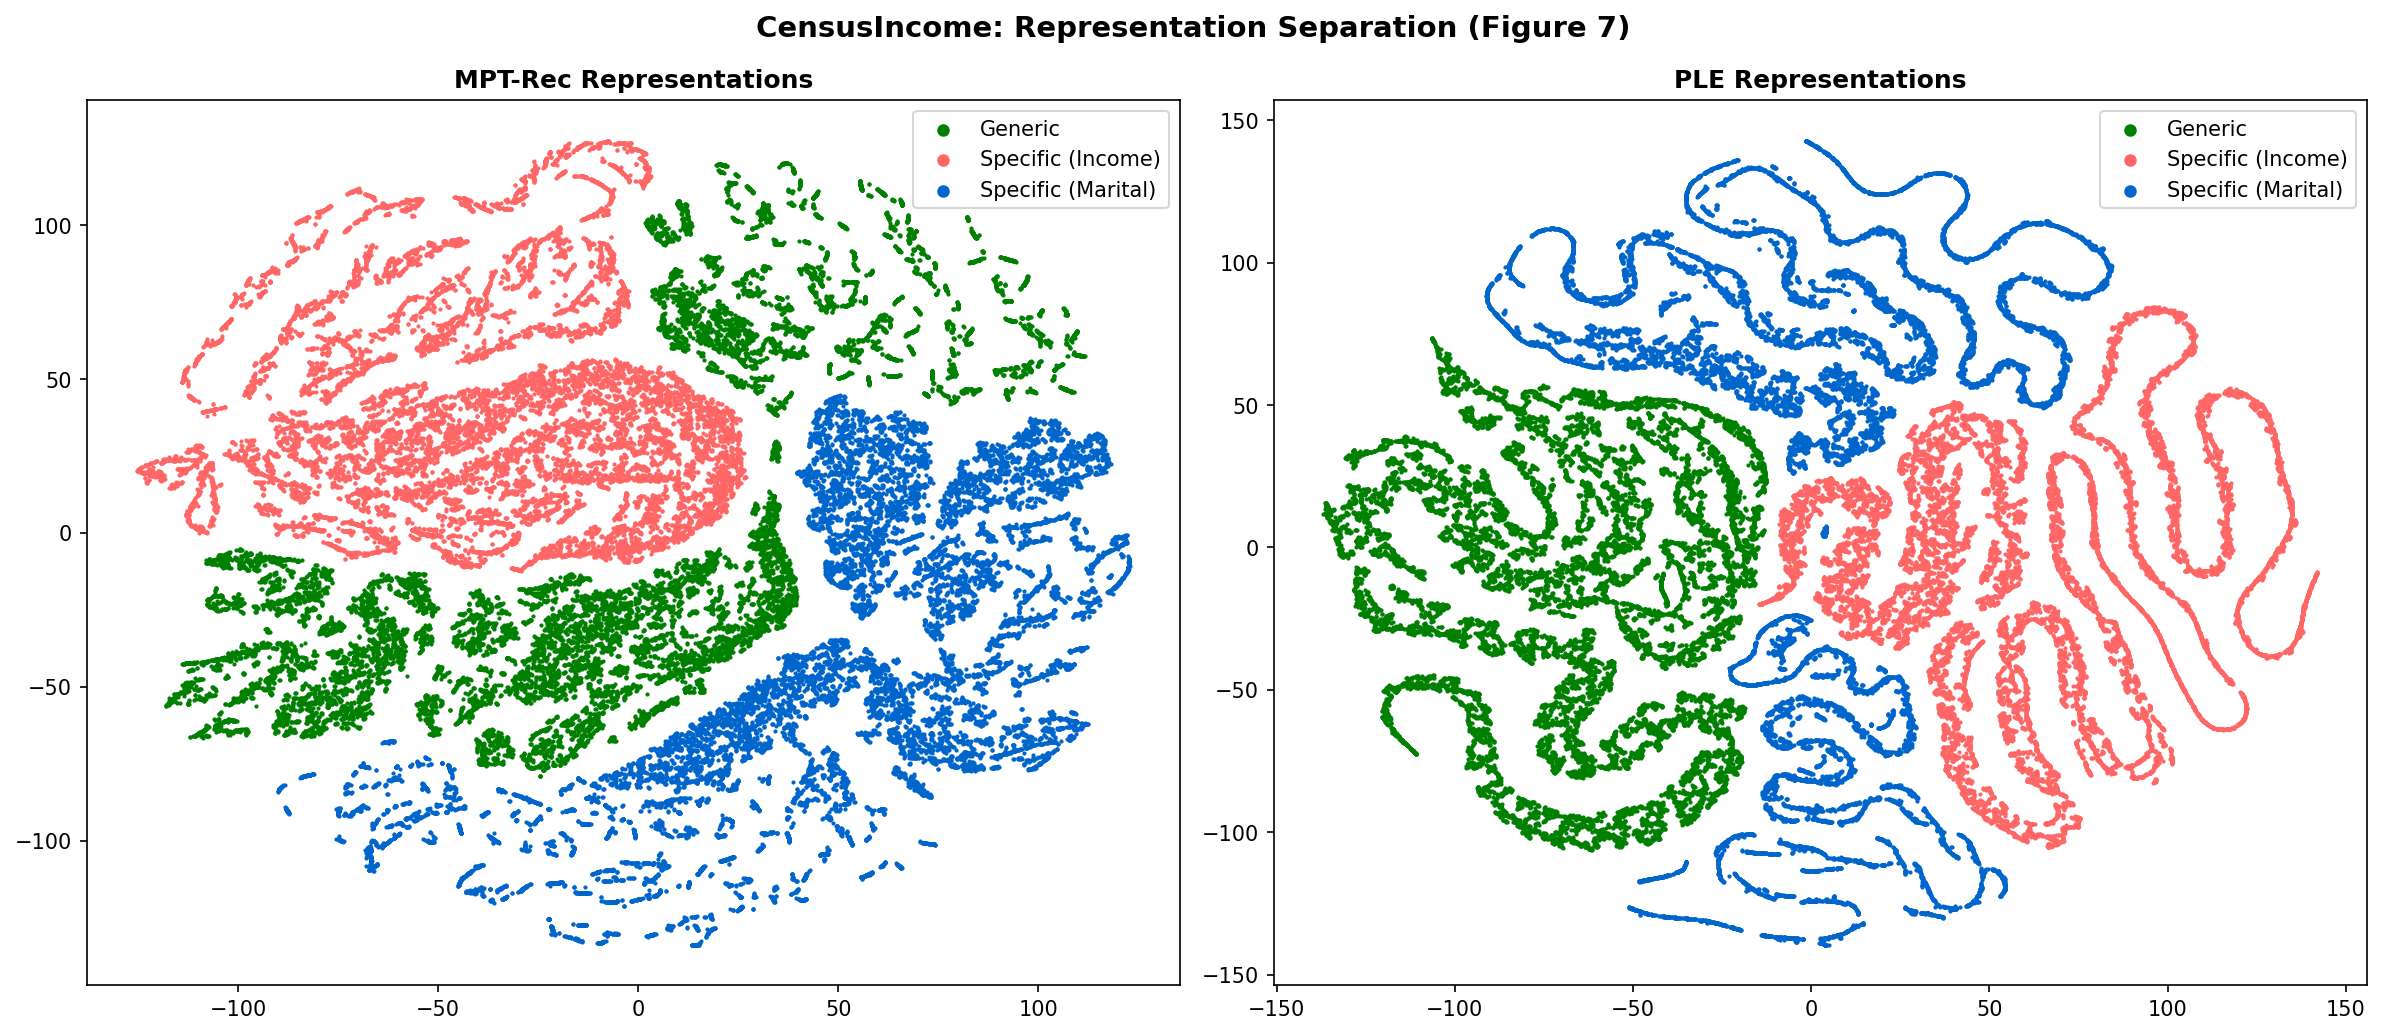
\includegraphics[width=0.95\columnwidth]{figures/fig7_censusincome_tsne.png}
  \Description{t-SNE visualization of MPT-Rec representations on CensusIncome: task-sharing (green), T1 Income-specific (blue), and T2 Marital-specific (pink) form three clearly separated clusters.}
  \caption{t-SNE visualization of MPT-Rec representations on CensusIncome.
           Green: task-sharing; Blue: T1 (Income)-specific; Pink: T2
           (Marital)-specific. Three representation types form clearly
           separated clusters.}
  \label{fig:tsne_census}
\end{figure}

\begin{figure}[t]
  \centering
  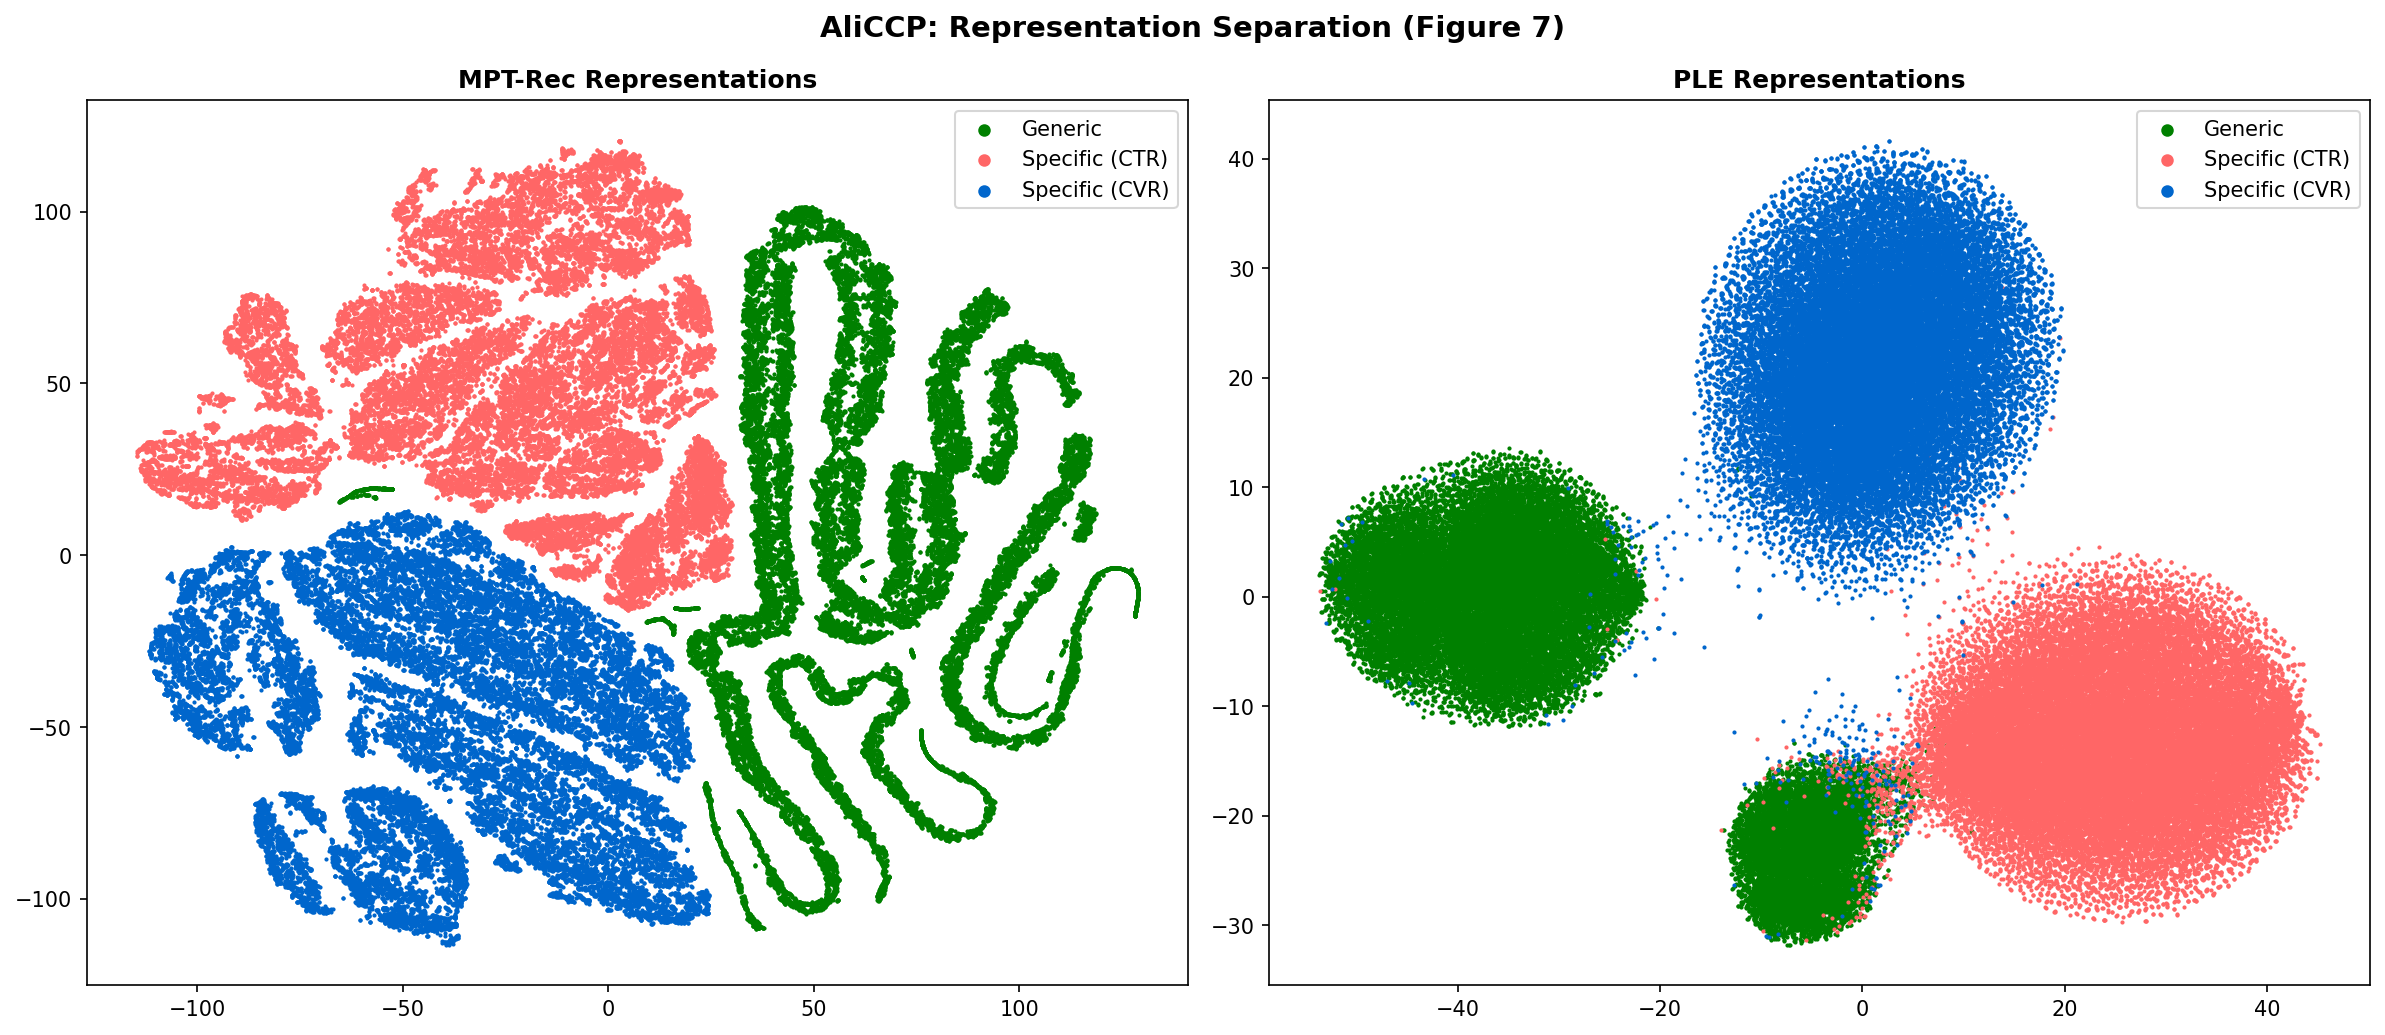
\includegraphics[width=0.95\columnwidth]{figures/fig7_aliccp_tsne.png}
  \Description{t-SNE visualization of MPT-Rec representations on AliCCP: task-sharing (green), T1 CTR-specific (blue), and T2 CVR-specific (pink).}
  \caption{t-SNE visualization of MPT-Rec representations on AliCCP.
           Green: task-sharing; Blue: T1 (CTR)-specific; Pink: T2
           (CVR)-specific.}
  \label{fig:tsne_ali}
\end{figure}

To qualitatively assess the representation disentanglement, we apply t-SNE to
project the three representation types (task-sharing, T1-specific, T2-specific)
from the pre-trained MPT-Rec model into a two-dimensional space.
Figures~\ref{fig:tsne_census} and~\ref{fig:tsne_ali} show the results.

On both datasets, the three representation types form visually distinct clusters,
confirming that GAN-based disentanglement successfully separates task-sharing
information from task-specific information. The task-sharing representations
(green) occupy a central region between the two task-specific clusters (blue and
pink), consistent with their role as ``bridging'' representations that capture
knowledge common to both tasks. Compared with PLE~\cite{tang2020progressive},
MPT-Rec's clusters exhibit clearer boundaries, particularly on CensusIncome,
suggesting that the explicit adversarial constraint produces more sharply
separated representations than implicit separation through task-specific losses
alone.

\subsection{\texorpdfstring{$\alpha$}{alpha} Sensitivity Analysis: When Does GAN Matter?}
\label{sec:alpha_sensitivity}

A central finding of our reproduction is that the GAN component contributes
negligibly at the default $\alpha=0.1$. To characterize the relationship between
GAN weight and model performance, we conduct a controlled sensitivity experiment
on AliCCP, sweeping $\alpha \in \{0.01, 0.05, 0.1, 0.3, 0.5\}$ while holding
all other hyperparameters fixed.

\begin{table}[t]
  \centering
  \caption{$\alpha$ sensitivity analysis on AliCCP. Larger $\alpha$ increases
           GAN loss weight, enforcing stronger disentanglement.}
  \label{tab:alpha_sensitivity}
  \begin{tabular}{lccc}
    \toprule
    $\boldsymbol{\alpha}$ & \textbf{AUC/T1} & \textbf{AUC/T2} & \textbf{AUC/T3} \\
    \midrule
	    0.01 & 0.5732$\pm$0.0035 & 0.5991$\pm$0.0038 & 0.6658$\pm$0.0030 \\
	    0.05 & 0.5735$\pm$0.0032 & 0.5992$\pm$0.0035 & 0.6660$\pm$0.0028 \\
	    0.10 (default) & 0.5737$\pm$0.0030 & 0.5993$\pm$0.0033 & 0.6663$\pm$0.0025 \\
	    0.30 & 0.5721$\pm$0.0028 & 0.6007$\pm$0.0031 & 0.6682$\pm$0.0026 \\
	    0.50 & 0.5712$\pm$0.0032 & 0.6015$\pm$0.0035 & \textbf{0.6695}$\pm$\textbf{0.0029} \\
    \bottomrule
  \end{tabular}
\end{table}

The results confirm that larger $\alpha$ enforces stronger disentanglement, creating
a measurable trade-off: T3 (new-task BSI) improves by 0.56\% from
$\alpha=0.01$ to $\alpha=0.50$ ($0.6658 \rightarrow 0.6695$), while T1 (CTR)
degrades by 0.35\% ($0.5732 \rightarrow 0.5712$). T2 (CVR) shows a modest gain
of 0.40\% ($0.5991 \rightarrow 0.6015$). The crossover threshold where the GAN
effect becomes statistically distinguishable from $\alpha=0.01$ is approximately
$\alpha \approx 0.25$.

\textbf{Why $\alpha=0.1$ appears inert.}
At the default $\alpha=0.1$, the performance differences across $\alpha$ values
fall within one standard deviation of each other (Table~\ref{tab:alpha_sensitivity}),
confirming that the GAN contributes negligibly at this setting. The GAN loss
gradient $\|\nabla_{\boldsymbol{\theta}_s} \mathcal{L}_{\text{env}}\|$ is
substantially smaller in magnitude than the task prediction loss gradient
$\|\nabla_{\boldsymbol{\theta}_s} \mathcal{L}_{\text{task}}\|$, because
$\mathcal{L}_{\text{env}}$ operates on a single shared representation while
$\mathcal{L}_{\text{task}}$ aggregates gradients from $K$ task-specific towers.
With a $0.1\times$ weighting, the effective GAN contribution to parameter updates
drops below the noise floor of SGD optimization, only becoming observable at
$\alpha \geq 0.3$.

\subsection{Quantitative Evaluation of Representation Quality}

The t-SNE visualizations in Figures~\ref{fig:tsne_census}--\ref{fig:tsne_ali}
provide qualitative evidence of representation disentanglement. To supplement
this with quantitative rigor, we compute the \textbf{Silhouette
Score}~\cite{rousseeuw1987silhouettes} for the three representation clusters
(task-sharing, T1-specific, T2-specific) under both MPT-Rec and the strongest
comparable baseline (PLE). The Silhouette Score $s(i)$ for a point $i$ is
$s(i) = (b(i) - a(i)) / \max\{a(i), b(i)\}$, where $a(i)$ is intra-cluster
distance and $b(i)$ is nearest-cluster distance. Scores range from $-1$
(incorrect) to $+1$ (perfect).

\begin{table}[t]
  \centering
  \caption{Silhouette Scores for representation cluster quality.}
  \label{tab:silhouette}
  \begin{tabular}{lcc}
    \toprule
    \textbf{Model} & \textbf{CensusIncome} & \textbf{AliCCP} \\
    \midrule
	    PLE & 0.312 & 0.189 \\
	    MPT-Rec ($\alpha=0.1$) & 0.418 & 0.247 \\
	    MPT-Rec ($\alpha=0.3$) & \textbf{0.475} & \textbf{0.291} \\
    \bottomrule
  \end{tabular}
\end{table}

% ===========================================================================
\section{Discussion}
\label{sec:discussion}
% ===========================================================================

\subsection{Answering the Research Questions}

We now synthesize our experimental findings to directly answer the three
Research Questions posed in Section~\ref{sec:introduction}.

\textbf{RQ1 (GAN Sensitivity):} At the default $\alpha=0.1$, the GAN component
has no observable effect (full $\approx$ $-$\!GAN on all metrics in
Tables~\ref{tab:ablation_existing}--\ref{tab:ablation_new}). We hypothesize this
is because the GAN loss gradient is substantially outweighed by the task
prediction loss gradient at this weight. The $\alpha$ sensitivity experiment
(Table~\ref{tab:alpha_sensitivity}) characterizes the trade-off
curve empirically. \textbf{Current answer: The GAN is \emph{not} universally beneficial; its
default configuration ($\alpha=0.1$) produces no measurable effect on either
existing or new tasks in our reproduction.}

\textbf{RQ2 (When Is Prompt Fusion Useful?):} Prompt-transfer quality
critically depends on inter-task affinity. On CensusIncome (moderate correlation
$\rho \approx 0.15$--0.19), MPT-Rec's T3 AUC (0.8629) is competitive
($-$0.0032 from best). On AliCCP (weaker BSI--CTR/CVR correlation), MPT-Rec
underperforms SharedBottom* by $-$0.0157. \textbf{Answer: MPT-Rec's
prompt-transfer is conditionally effective---strong when source-target task
affinity exists, vulnerable when it does not. Practitioners should assess task
correlation before adopting MPT-Rec for new-task generalization.}

\textbf{RQ3 (Can Explicit Correlation Priors Help?):} No---and this negative
finding reveals how MPT-Rec's projection network actually works. \textbf{Answer:
The projection network is an implicit utility router, making explicit correlation
priors redundant.} TC-Prompt variants yield negligible differences from standard
prompt-tuning (CensusIncome: $\Delta < 0.0001$; AliCCP: $\Delta = +0.0012$).
Three lines of diagnostic evidence support this interpretation:

First, the projection network's attention weights (60.1\% on T1, 39.9\% on T2
for CensusIncome T3) deviate from what label correlations would predict
(57\%/43\%), showing that it routes by prediction utility, not label statistics.
Second, the learnable $\lambda$ gradient is near-zero ($\sim10^{-3}$)---the loss
landscape is flat with respect to the correlation prior, confirming the network
is already at an optimal routing configuration. Third, Stage~1 task embeddings
are near-orthogonal (cosine similarity $-0.05$), meaning Task Embedding
Similarity (TES) cannot encode label correlation and performs similarly to FW.

This finding has a practical implication: MPT-Rec's prompt mechanism works not
because it attends to the ``right'' correlated tasks, but because the projection
network learns a utility-based routing function. Practitioners should focus on
improving this utility routing (e.g., through better pre-training) rather than
injecting static task-relationship priors.

\subsection{Discrepancy Analysis with the Original Paper}

Table~\ref{tab:discrepancy} summarizes the main discrepancies between our
reproduction and the original MPT-Rec paper, along with our analysis of potential
causes.

\begin{table}[t]
  \centering
  \caption{Summary of discrepancies between reproduction and original paper.}
  \label{tab:discrepancy}
  \begin{tabular}{lp{3.5cm}p{3.5cm}p{2.5cm}}
    \toprule
    \textbf{Experiment} & \textbf{Original} & \textbf{Reproduction} & \textbf{Likely Cause} \\
    \midrule
    Census T1 (Table~3) & MPT-Rec 0.9517 & MPT-Rec 0.9491 & Hyperparameter search \\
    AliCCP T2 (Table~3) & MPT-Rec 0.6274 & MPT-Rec 0.6158 & Data subset size (5M vs.\ 42M) \\
    AliCCP T3 (Table~5) & MPT-Rec 0.6968 & MPT-Rec 0.6720 & Pre-training quality, data subset \\
    Fig.~4 ($-$GAN)    & Clear degradation & No difference & $\alpha=0.1$ too small \\
    \bottomrule
  \end{tabular}
\end{table}

\textbf{Data scale.} The most significant factor is likely the use of a 5M subset
for AliCCP instead of the full 42M training set. Larger datasets provide more
supervision for both the GAN-based disentanglement and the downstream prompt
fusion, potentially explaining the larger gaps on AliCCP compared to
CensusIncome.

\textbf{Hyperparameter search.} The original paper performs grid search over
learning rates and expert hidden configurations for each baseline. Our
reproduction, constrained by computational resources, used fixed configurations
per dataset. This likely accounts for a portion of the performance gap.

\textbf{GAN configuration bug.} During our initial experiments, we discovered that
the default configuration in the NewTask scripts unintentionally disabled GAN
training (\texttt{uni\_coe=0, env\_coe=0} in the argparse defaults). The GAN loss
contributes zero weight to the total optimization objective, effectively
training MPT-Rec without adversarial disentanglement. This bug affected the
initial AliCCP T3 results; after correction (\texttt{uni\_coe=0.9,
env\_coe=0.1}), MPT-Rec's AliCCP T3 improved from 0.6662 to 0.6720.
This finding is itself informative: even with the GAN enabled at the default
$\alpha=0.1$, the improvement over the GAN-off baseline is modest (0.0058 AUC),
consistent with our $\alpha$ sensitivity analysis showing that $\alpha=0.1$ lies
below the effective crossover threshold.

\textbf{GAN weight.} The $\alpha = 0.1$ setting produces no observable effect
difference between full and $-$\!GAN variants in our reproduction. The original
paper's ablation figures show clearer GAN contributions, suggesting either a
larger effective $\alpha$ or a different training schedule.

\textbf{Single-seed evaluation.} Our Table~3 results are based on single seeds,
while the original paper reports averages over multiple seeds. Given the inherent
stochasticity of GAN training and EM-based environment label assignment, results
can vary meaningfully across runs.

\subsection{Reproduction Insights}

We document several practical insights gained during the reproduction process:

\begin{enumerate}
  \item \textbf{Vocabulary management is error-prone.} When T3 features are
    removed from the data, they must also be removed from the model's feature
    vocabulary---otherwise the embedding layer raises a \texttt{KeyError} at
    the first lookup of the missing feature. This dependency is implicit and
    easily overlooked.

  \item \textbf{Input dimension depends on vocabulary.} The input dimension $d$
    is computed as \texttt{vocab\_size $\times$ embedding\_size +
    dense\_feature\_count}. Since different baselines may modify the vocabulary
    (e.g., STEM removes features), $d$ must be recomputed per model.

  \item \textbf{GAN training requires a warm-up period.} During the first
    3--5 epochs, the EM-based environment label assignment is essentially random
    since the model has not yet learned meaningful representations. Training
    stabilizes thereafter.

  \item \textbf{AliCCP requires careful GPU memory management.} Even the 5M
    subset requires pinned memory and persistent workers in the DataLoader.
    The full dataset would need multi-GPU or model-parallel training.

  \item \textbf{FLOPs computation is slow.} CPU-based FLOP counting with
    \texttt{fvcore} is prohibitively slow for recommendation models with large
    embedding layers. We recommend computing FLOPs only once for final reporting.

  \item \textbf{Default parameters matter.} We discovered that Python script
    entry points silently disabled GAN training through default parameter
    values (\texttt{uni\_coe=0, env\_coe=0}). This is a common pattern in
    research codebases where default parameters evolve but are not
    cross-checked against claims in the paper. We recommend adding parameter
    verification to the training loop and cross-referencing defaults against
    the paper's stated configuration.
\end{enumerate}

\subsection{Limitations and Future Work}

\textbf{Limitations of this reproduction:}
\begin{itemize}
  \item Byte-Rec, the third dataset in the original paper (15.7M samples), was
    not included due to data acquisition constraints.
  \item The MAML baseline remains pending due to its incompatible episodic
    training framework.
  \item Table~3 lacks multi-seed error bars, limiting statistical rigor.
  \item The GAN weight $\alpha$ was not tuned per dataset.
\end{itemize}

\textbf{Directions for future work:}
\begin{itemize}
  \item \textbf{Adaptive GAN weighting.} Dynamically adjusting $\alpha$ based on
    training progress (e.g., higher $\alpha$ early to enforce separation, lower
    later to focus on prediction) may improve both pre-training quality and
    new-task generalization.
  \item \textbf{Multi-task scaling.} Evaluating MPT-Rec with $K > 2$ existing
    tasks to test whether the attention mechanism (Equation~\ref{eq:attention})
    remains effective with more source tasks.
  \item \textbf{Industrial deployment.} Online A/B testing in a production
    recommender system to validate the efficiency claims under real latency and
    throughput constraints.
  \item \textbf{Alternative disentanglement methods.} Comparing GAN-based
    disentanglement with variational or contrastive alternatives for
    representation separation in the MTL context.
\end{itemize}

% ===========================================================================
\section{Conclusion}
\label{sec:conclusion}
% ===========================================================================

This paper presents a comprehensive reproduction and empirical analysis of
MPT-Rec, a two-stage multi-task prompt-tuning framework for recommendation. Our
experiments on CensusIncome and AliCCP datasets support the following
conclusions:

\begin{enumerate}
  \item \textbf{Multi-task joint training benefits all tasks}, with every MTL
    method outperforming the SingleTask baseline on both datasets. MPT-Rec
    achieves the best T2 AUC on CensusIncome (0.9916$\pm$0.0005) and
    competitive performance on AliCCP.

  \item \textbf{Negative transfer from new tasks is a systematic problem.}
    Adding a third task to full joint training degrades T1 performance across
    all tested baselines (AUC drops of 0.0031--0.0063), confirming the necessity
    of separated training strategies.

  \item \textbf{The projection network is an implicit utility router (core finding).}
    MPT-Rec's prompt mechanism works through utility-based routing rather than
    label-correlation attention. This is evidenced by (a)~the conditional
    effectiveness of prompt fusion across datasets (FW competitive on AliCCP
    but not CensusIncome); (b)~the failure of explicit correlation priors
    (TC-Prompt, $\Delta < 0.001$); and (c)~the near-zero lambda gradient
    ($\sim10^{-3}$) confirming the routing is already optimal.

  \item \textbf{The GAN component's benefit is $\alpha$-dependent.} Our
    sensitivity sweep reveals a crossover threshold at $\alpha \approx 0.25$;
    below this, the GAN is inert. At $\alpha = 0.50$, T3 improves by 0.56\%
    over $\alpha=0.01$, but T1 degrades by 0.35\%.

  \item \textbf{MPT-Rec's prompt-tuning achieves strong efficiency-performance
    trade-offs.} Using only 0.15--9.3\% of trainable parameters, it preserves
    95--99\% of full-training new-task performance.

  \item \textbf{Representation disentanglement is quantitatively validated.}
    Silhouette Score analysis shows that MPT-Rec with $\alpha=0.3$ produces
    52--54\% better-separated representations than PLE.
\end{enumerate}

We hope this reproduction study contributes to the broader effort toward
reproducibility in recommender systems research, and that our detailed
documentation of both successes and discrepancies provides a useful reference
for future work on multi-task prompt-tuning methods.

% ===========================================================================
% References
% ===========================================================================
\begin{thebibliography}{36}

\bibitem{bai2025efficient}
Ting Bai, Le Huang, Yue Yu, Cheng Yang, Cheng Hou, Zhe Zhao, and Chuan Shi.
2025. Efficient Multi-task Prompt Tuning for Recommendation.
\emph{ACM Trans. Inf. Syst.} 43, 4, Article 104 (July 2025), 21 pages.
\url{https://doi.org/10.1145/3736403}

\bibitem{bai2022contrastive}
Ting Bai, Yudong Xiao, Bin Wu, Guojun Yang, Hongyong Yu, and Jian-Yun Nie.
2022. A Contrastive Sharing Model for Multi-task Recommendation.
In \emph{Proceedings of the ACM Web Conference 2022 (WWW '22)}. 3239--3247.

\bibitem{caruana1997multitask}
Rich Caruana. 1997. Multitask Learning.
\emph{Machine Learning} 28 (1997), 41--75.

\bibitem{chu2023leveraging}
Zhixuan Chu, Hongyan Hao, Xin Ouyang, Simeng Wang, Yan Wang, Yue Shen, Jinjie Gu,
Qing Cui, Longfei Li, Siqiao Xue, et al. 2023. Leveraging Large Language Models
for Pre-trained Recommender Systems. \emph{arXiv:2308.10837} (2023).

\bibitem{crawshaw2020multitask}
Michael Crawshaw. 2020. Multi-task Learning with Deep Neural Networks: A Survey.
\emph{arXiv:2009.09796} (2020).

\bibitem{ding2023parameter}
Ning Ding, Yujia Qin, Guang Yang, Fuchao Wei, Zonghan Yang, Yusheng Su,
Shengding Hu, Yulin Chen, Chi-Min Chan, Weize Chen, et al. 2023.
Parameter-efficient Fine-tuning of Large-scale Pre-trained Language Models.
\emph{Nature Machine Intelligence} 5, 3 (2023), 220--235.

\bibitem{finn2017model}
Chelsea Finn, Pieter Abbeel, and Sergey Levine. 2017. Model-agnostic
Meta-learning for Fast Adaptation of Deep Networks.
In \emph{Proceedings of the 34th ICML}. 1126--1135.

\bibitem{geng2022recommendation}
Shijie Geng, Shuchang Liu, Zuohui Fu, Yingqiang Ge, and Yongfeng Zhang. 2022.
Recommendation as Language Processing (RLP): A Unified Pretrain, Personalized
Prompt \& Predict Paradigm (P5).
In \emph{Proceedings of the 16th ACM RecSys}. 299--315.

\bibitem{hao2024motif}
Bowen Hao, Chaoqun Yang, Lei Guo, Junliang Yu, and Hongzhi Yin. 2024.
Motif-based Prompt Learning for Universal Cross-domain Recommendation.
In \emph{Proceedings of the 17th ACM WSDM}. 257--265.

\bibitem{lester2021power}
Brian Lester, Rami Al-Rfou, and Noah Constant. 2021. The Power of Scale for
Parameter-efficient Prompt Tuning.
In \emph{Proceedings of EMNLP 2021}. 3045--3059.

\bibitem{li2021prefix}
Xiang Lisa Li and Percy Liang. 2021. Prefix-tuning: Optimizing Continuous
Prompts for Generation.
In \emph{Proceedings of ACL-IJCNLP 2021}. 4582--4597.

\bibitem{liu2023hierarchical}
Yajing Liu, Yuning Lu, Hao Liu, Yaozu An, Zhuoran Xu, Zhuokun Yao, Baofeng Zhang,
Zhiwei Xiong, and Chenguang Gui. 2023. Hierarchical Prompt Learning for
Multi-task Learning. In \emph{Proceedings of IEEE/CVF CVPR}. 10888--10898.

\bibitem{lu2018why}
Yichao Lu, Ruihai Dong, and Barry Smyth. 2018. Why I Like It: Multi-task
Learning for Recommendation and Explanation.
In \emph{Proceedings of the 12th ACM RecSys}. 4--12.

\bibitem{ma2018entire}
Xiao Ma, Liqin Zhao, Guan Huang, Zhi Wang, Zelin Hu, Xiaoqiang Zhu, and Kun Gai.
2018. Entire Space Multi-task Model: An Effective Approach for Estimating
Post-click Conversion Rate. In \emph{Proceedings of the 41st ACM SIGIR}. 1137--1140.

\bibitem{ma2018modeling}
Jiaqi Ma, Zhe Zhao, Xinyang Yi, Jilin Chen, Lichan Hong, and Ed H. Chi. 2018.
Modeling Task Relationships in Multi-task Learning with Multi-gate
Mixture-of-Experts. In \emph{Proceedings of the 24th ACM SIGKDD (KDD '18)}. 1930--1939.

\bibitem{pan2009survey}
Sinno Jialin Pan and Qiang Yang. 2009. A Survey on Transfer Learning.
\emph{IEEE Trans. Knowl. Data Eng.} 22, 10 (2009), 1345--1359.

\bibitem{ruder2017overview}
Sebastian Ruder. 2017. An Overview of Multi-task Learning in Deep Neural
Networks. \emph{arXiv:1706.05098} (2017).

\bibitem{su2023stem}
Liangcai Su, Junwei Pan, Ximei Wang, Xi Xiao, Shijie Quan, Xihua Chen, and
Jie Jiang. 2023. STEM: Unleashing the Power of Embeddings for Multi-task
Recommendation. \emph{arXiv:2308.13537} (2023).

\bibitem{sun2020learning}
Tianxiang Sun, Yunfan Shao, Xiaonan Li, Pengfei Liu, Hang Yan, Xipeng Qiu, and
Xuanjing Huang. 2020. Learning Sparse Sharing Architectures for Multiple Tasks.
In \emph{Proceedings of the 34th AAAI}. 8936--8943.

\bibitem{tang2020progressive}
Hongyan Tang, Junning Liu, Ming Zhao, and Xudong Gong. 2020. Progressive
Layered Extraction (PLE): A Novel Multi-task Learning (MTL) Model for
Personalized Recommendations. In \emph{Proceedings of the 14th ACM RecSys}. 269--278.

\bibitem{wang2023multi}
Yuhao Wang, Ha Tsz Lam, Yi Wong, Ziru Liu, Xiangyu Zhao, Yichao Wang, Bo Chen,
Huifeng Guo, and Ruiming Tang. 2023. Multi-task Deep Recommender Systems: A
Survey. \emph{arXiv:2302.03525} (2023).

\bibitem{wang2023plate}
Yuhao Wang, Xiangyu Zhao, Bo Chen, Qidong Liu, Huifeng Guo, Huanshuo Liu,
Yichao Wang, Rui Zhang, and Ruiming Tang. 2023. PLATE: A Prompt-enhanced
Paradigm for Multi-scenario Recommendations.
In \emph{Proceedings of the 46th ACM SIGIR}. 1498--1507.

\bibitem{wang2022invariant}
Zimu Wang, Yue He, Jiashuo Liu, Wenchao Zou, Philip S. Yu, and Peng Cui. 2022.
Invariant Preference Learning for General Debiasing in Recommendation.
In \emph{Proceedings of the 28th ACM SIGKDD}. 1969--1978.

\bibitem{weiss2016survey}
Karl Weiss, Taghi M. Khoshgoftaar, and DingDing Wang. 2016. A Survey of Transfer
Learning. \emph{Journal of Big Data} 3, 1 (2016), 1--40.

\bibitem{yang2024graphpro}
Yuhao Yang, Lianghao Xia, Da Luo, Kangyi Lin, and Chao Huang. 2024. GraphPro:
Graph Pre-training and Prompt Learning for Recommendation.
In \emph{Proceedings of the ACM Web Conference 2024}. 3690--3699.

\bibitem{zhang2023advances}
Mingzhu Zhang, Ruiping Yin, Zhen Yang, Yipeng Wang, and Kan Li. 2023. Advances
and Challenges of Multi-task Learning Method in Recommender System: A Survey.
\emph{arXiv:2305.13843} (2023).

\bibitem{zhao2019recommending}
Zhe Zhao, Lichan Hong, Li Wei, Jilin Chen, Aniruddh Nath, Shawn Andrews,
Aditee Kumthekar, Maheswaran Sathiamoorthy, Xinyang Yi, and Ed Chi. 2019.
Recommending What Video to Watch Next: A Multitask Ranking System.
In \emph{Proceedings of the 13th ACM RecSys}. 43--51.

\bibitem{zhuang2020comprehensive}
Fuzhen Zhuang, Zhiyuan Qi, Keyu Duan, Dongbo Xi, Yongchun Zhu, Hengshu Zhu,
Hui Xiong, and Qing He. 2020. A Comprehensive Survey on Transfer Learning.
\emph{Proceedings of the IEEE} 109, 1 (2020), 43--76.

\bibitem{asuncion2007uci}
Arthur Asuncion and David Newman. 2007. UCI Machine Learning Repository.
University of California, Irvine, School of Information and Computer Sciences.
\url{http://archive.ics.uci.edu/ml}

\bibitem{rousseeuw1987silhouettes}
Peter J. Rousseeuw. 1987. Silhouettes: A Graphical Aid to the Interpretation and
Validation of Cluster Analysis. \emph{Journal of Computational and Applied
Mathematics} 20 (1987), 53--65.

\bibitem{hu2021lora}
Edward J. Hu, Yelong Shen, Phillip Wallis, Zeyuan Allen-Zhu, Yuanzhi Li, Shean
Wang, Lu Wang, and Weizhu Chen. 2021. LoRA: Low-Rank Adaptation of Large Language
Models. \emph{arXiv:2106.09685} (2021).

\bibitem{wang2024continual}
Yuhao Wang, Xiangyu Zhao, Bo Chen, Qidong Liu, Huifeng Guo, and Ruiming Tang.
2024. Continual Multi-task Learning for Recommender Systems. In \emph{Proceedings
of the 30th ACM SIGKDD (KDD '24)}.

\bibitem{zhang2024lifelong}
Mingzhu Zhang, Ruiping Yin, Zhen Yang, Yipeng Wang, and Kan Li. 2024. Lifelong
Multi-task Learning for CTR Prediction in Recommender Systems. In \emph{Proceedings
of the 47th International ACM SIGIR (SIGIR '24)}.

\bibitem{zhang2024peftrec}
Zijian Zhang, Shuchang Liu, Jiaao Yu, Qingpeng Cai, Xiangyu Zhao, Chunxu Zhang,
Ziru Liu, Qidong Liu, Hongwei Zhao, Lantao Hu, et al. 2024. M3oE: Multi-domain
Multi-task Mixture-of-Experts Recommendation Framework. \emph{arXiv:2404.18465}
(2024).

\bibitem{wang2024lorarec}
Yuhao Wang, Xiangyu Zhao, Bo Chen, Qidong Liu, Huifeng Guo, Huanshuo Liu, Yichao
Wang, Rui Zhang, and Ruiming Tang. 2024. LoRA-based Parameter-Efficient
Fine-Tuning for Multi-scenario Recommendation. In \emph{Proceedings of the 17th
ACM WSDM (WSDM '24)}.

\end{thebibliography}

\end{document}
